% #############################################################################
% This is Appendix Assertiveness-based Details (CHI 2023)
% !TEX root = main.tex
% #############################################################################
\chapter{Assertiveness-based Details}
\label{chap:app005}

In this appendix, we provide additional details from Chapter~\ref{chap:chap006} on the use of \ac{AI} models in our \ac{UI}, as well as the severity classification during patient diagnosis, our patient selection, and information about participants.
We also discuss the existing system, evaluating performance recognition, thresholds, and strategies for curating patients, the following steps for explanations and tone, and the repositories.
As follows, we will provide further information to understand the details of our work better.

\section{Extended Motivation}
\label{sec:app005001}

\ac{AI} systems are showing increasing promise for numerous healthcare applications.
Recently, the advantages of \ac{DL} are spawning \ac{AI} systems with human-like performance in several clinical domains~\cite{CALISTO2022102285, Hannun2019, Ruamviboonsuk2019}.
However, these applications are not designed to capture the variability of personal or subpopulation level of clinicians~\cite{Uddin2019}.
Recent works highlight how \ac{AI} and the advancement of technologies together are empowering the aim of personalized and precision medicine~\cite{HO2020497, Wetzstein2020}.
Given the need to personalize and customize the \ac{AI} recommendations, an essential question in the design of \ac{AI} systems is how they should communicate, considering the professional experience of the clinician.

To achieve a more persuasive and reliable intelligent agent, we must analyze and collect data regarding the clinician's behavior~\cite{PELAU2021106855}.
Communication is essential to increase the reliability of an intelligent agent~\cite{10.1145/3311350.3347162} providing a diagnosis to a clinician.
One way to achieve that is by aligning the levels of assertiveness~\cite{pacheco2019alignment} of the agent with the years of experience of the clinician.
Besides that, explaining `how' and `why' the \ac{AI} assistant achieved a particular output increases trust in the system, solving a problem known as the ``black-box'' problem~\cite{10.1145/3491102.3502104, CALISTO2021102607}.

In this appendix, we present further details of our study for applying {\it BreastScreening-AI} prototype (Section~\ref{sec:chap005004} of Chapter~\ref{chap:chap005}) in two conditions, where clinicians will interact with conventional and assertiveness-based intelligent agents~\cite{pacheco2019alignment, 10.1145/3311350.3347162}.
The assistant will act as a second reader, resulting in improvements in diagnostic performance, by reducing \acp{FP} and \acp{FN} ({\it i.e.}, Over-Diagnosis {\it vs} Under-Diagnosis), as well as inefficiency and efficacy in the clinical workflow (Section~\ref{sec:chap006006001}).
While considerable work has focused on improving the accuracy of \ac{AI} algorithms, comparatively less work focused on improving the adoption and usability of interactive assistance techniques.
This paper broadly examines what clinicians need when using \ac{AI}-powered assistance, the practices they adopt while using diagnostic tools, and how these tools affect end-user attitudes toward the underlying \ac{AI} algorithms.

Here, we detail a within-subject study with 52 clinicians who interacted with both conventional and assertiveness-based agents, diagnosing a total of 35 patients from a dataset of 289 patients, out of which 34\% have benign abnormalities, 31\% have malignant abnormalities, and the other 35\% are healthy patients (Section~\ref{sec:app005010}).
Two different tones were used to communicate the \ac{AI} recommendations in our assertiveness-based agent, from a more suggestive to a more imposing tone.
Moreover, the assertiveness-based agent explained `{\it how}' and `{\it why}' the \ac{AI} algorithms achieved a particular diagnostic by providing human-interpretable clinical arguments for the achieved outputs.

While we used actual \ac{AI} outputs and clinical arguments curated from human clinicians, the \ac{AI} models were trained for classification and segmentation purposes through different architectures.
Specifically, through a DenseNet model~\cite{8721151} for a multimodal diagnosis of \ac{MG} and \ac{US} images.
Similarly, a 3D ResNet model~\cite{Aldoj2020} was trained to diagnose the \ac{MRI} volumes.
Our findings suggest that explaining the \ac{AI} outputs and clinical arguments by exploring how to adapt the communication through an assertiveness-based agent can benefit \ac{AI} assistance of medical reasoning.

The novelty of this work lies in applying communication theories through \ac{DL} systems to investigate the impact of assertiveness-based \ac{AI} mediation on different expertise levels in critical medical decision-making.
To achieve this, we updated the design of the {\it BreastScreening-AI} framework~\cite{CALISTO2022102285} to examine how assertiveness-based communication influences different expertise levels in clinical scenarios.
Our contributions encompass knowledge in computational interaction approaches, specifically assertiveness-based \ac{AI} mediation in the \ac{HCI} field, as well as insights into designing interactive systems guided by computational principles for the \ac{CHI} community.

\section{Further Contributions}
\label{sec:app005002}

So far, we have provided an extended motivation (Section~\ref{sec:app005001}) with more information to sustain the work under Section~\ref{sec:chap006001} of Chapter~\ref{chap:chap006}.
In this section, we provide further details on the contributions of this work.
The work was published~\cite{10.1145/3544548.3580682} and {\it peer-reviewed} at the \acs{CHI} 2023 conference.

\vspace{0.50mm}

\noindent
In sum, the main contributions of this work are as follows:

\vspace{0.05mm}

\begin{enumerate}
\item We present a novel approach for personalizing and customizing \ac{AI}-assisted medical reasoning, providing evidence that assertiveness-based agents can alter clinical workflows by effectively adapting the communication depending on the categories of medical professional experience.
\item We demonstrate that while explaining the \ac{AI} outputs can enhance medical efficiency, its impact heavily depends on the communication tone ({\it i.e.}, more suggestive or imposing the \ac{AI} recommendations) of the provided clinical arguments.
\item We report our results demonstrating that these assertiveness-based agents can increase the utility of clinical information found and increase user trust in the \ac{AI} recommendations, without a loss in diagnostic performance.
\item We provide design considerations for adapting the communication in \ac{AI}-assisted medical reasoning, laying a foundation for future implementations of intelligent agents better capable of personalizing and customizing explanations.
\end{enumerate}

\vspace{0.05mm}

Across the following sections, we outline related works on the issues of guiding the \ac{HAII} topic, assisting decision-making, going through some examples of \acp{CDSSe} present in the literature~\cite{NAISEH2023102941, 10.1145/3531146.3533193}, and ending on the effects of \ac{AI} communication.
We then introduce the design of our {\it Assertiveness-based BreastScreening-AI} assistant, followed by our research questions, hypotheses, and methods.
Last, we report our quantitative and qualitative findings, as well as conclude with a discussion of design considerations.

\section{Additional Literature}
\label{sec:app005003}

This section covers additional literature from Section~\ref{sec:chap006002} of Chapter~\ref{chap:chap006} on medical imaging system integration, challenges in clinical decision-making, \acp{CDSSe}, and the effects of \ac{AI} communication. The intersection of cognitive psychology, learnability, and context awareness in \ac{HCI} is examined. Personalized and customized algorithmic suggestions based on medical expertise levels are highlighted, along with the impact of \ac{AI} communication on trust and decision-making. The focus is on studying how assertiveness-based \ac{AI} mediation affects clinicians with different levels of expertise.

Medical imaging systems play a crucial role in diagnosing various modalities, such as \ac{MG}, \ac{US}, and \ac{MRI}, by enabling seamless data retrieval.
Integrating these modalities offers opportunities for quantitative imaging and diagnoses, necessitating specialized data handling, post-processing, and visualization methods~\cite{Igarashi:2016:IVS:2984511.2984537}.
In the clinical domain, medical imaging tools assist experts in making more informed decisions, including identifying cancer prognostics using multi-modal data.

In this section, we provide additional literature from Section~\ref{sec:chap006002} that expands on integrating \ac{CDSSe} into the radiology workflow.
The selected works aim to explore different aspects and expectations, focusing on enhancing medical imaging diagnosis through assertiveness-based interaction.
These studies shed light on the potential benefits and challenges of incorporating assertiveness-based \ac{AI} systems in the clinical setting.

\subsection{Human-AI Interaction Details}
\label{sec:app005003001}

Intelligent agents need to provide users with, not only results, but also accounting for their behaviors during decision-making~\cite{10.1145/3313831.3376807}.
In the field of \ac{HCI}, the topic of \ac{XAI} contains subjects that intersect cognitive psychology, learnability, and context awareness~\cite{doi:10.1073/pnas.1618211113}.
Cognitive psychology is a subject focusing more on explanation theory.
For cognitive psychology, we know that cognitive explanations are strongly connected with causality reasoning~\cite{10.1145/3544548.3580682}.
Learnability is an important part of usability~\cite{CALISTO2021102607}.
Here, the literature summarized topics of learnability related to designing a \ac{XAI} system, such as hints, guidance, and visualizations~\cite{CALISTO2022102285}.
These aspects contribute to the understanding of how intelligent agents can effectively communicate and provide meaningful explanations in decision-making processes.

Explainable context awareness is a simplistic representation of the context to inform users what is obtained and which action will be done by the system~\cite{10.1145/3313831.3376545}.
Other authors~\cite{Kocielnik:2019:YAI:3290605.3300641} designed a tailored interface, providing visual and textual explanations following several context-aware rules.
However, research in both \ac{HCI} and \ac{AI} communities is often disconnected between the two fields~\cite{10.1145/3173574.3174156, 10.1145/3313831.3376807}.
There is a research gap that is not crossing nor combine both fields to the interdisciplinary approach of accounting user's different behavioral characteristics (Section~\ref{sec:chap003001} of Chapter~\ref{chap:chap003}) during decision-making~\cite{10.1145/3173574.3174156}.
Therefore, both \ac{HCI} and \ac{AI} communities need to bridge this gap with further collaboration and investigation for an understanding enhancement of \acp{HAII} in decision-making processes.

\ac{HAII} incorporates human feedback in the model training process to create better \ac{ML} models.
In this thesis, we refer to the topic as \ac{HAII}, which somehow is addressed by Amershi et al.~\cite{10.1145/3290605.3300233} providing a set of design guidelines~\cite{10.1145/3132272.3134111}.
The work of Kocielnik et al.~\cite{Kocielnik:2019:YAI:3290605.3300641} is also addressing the study on the impact of several methods of expectation setting, and others studied the design for specific \ac{HAII} scenarios~\cite{aha2017ai}.
While prior work relies on handcrafted features~\cite{10.1145/3290605.3300233, Kocielnik:2019:YAI:3290605.3300641}, our approach leverages rich image data features automatically learned from \ac{DL} algorithms by adapting the outcomes to the {\it end-user}.
Specifically, we focus on personalized and customized \ac{AI} suggestions tailored to varying levels of medical expertise.

Many researchers have argued that \ac{HAII} would be improved if the \ac{AI} systems could {\it explain their reasoning}~\cite{10.1145/3411764.3445717, Rudin2022, Kawamleh2022}.
In medicine, explaining predictions from \ac{AI} models is particularly salient, where the uncovered patterns of the model can be more important than prediction performance~\cite{Lundberg2020}.
The literature demonstrates how to retain interpretability by developing a method to provide explanations of model predictions~\cite{10.1145/3544548.3580682}.
Although these works explore how clinicians interact with \ac{AI} recommendations and their perceptions of \ac{AI} outcomes, they are not taking into account cognitive bias in decision-making.
One of the most notorious cognitive differences is seen between people with different levels of expertise and knowledge~\cite{https://doi.org/10.1111/nuf.12430, Seidel2021}.
We are studying how assertiveness-based agents are designed to adapt their communication tone based on expertise levels to reduce cognitive bias.

\subsection{Assisting Clinical Decision-Making}
\label{sec:app005003002}

Although the research in interaction with intelligent agents is recent, still this topic has seen new advances, {\it e.g.}, chat-bots and other agents~\cite{miller2019intrinsically}.
Recent advances in medical technologies that promote data generation have continued to drive interaction research in the clinical domain~\cite{azuaje2019artificial, Lopes:2017:UHC:3143820.3144118}.
Moreover, the new interest of the medical community to support \ac{AI} research projects and the available public {\it datasets}, are encouraging researchers to work in both fields~\cite{lau2018dataset}.
Therefore, we bring together both \ac{HCI} and \ac{AI} communities to leverage the high-stakes of clinical decision-making.

The introduction of technology for assisting clinical decision-making is fraught with challenges and unintended consequences, such as critical decisions dealing with patient safety, clinician fatigue, and increased medical errors~\cite{10.1093/jamia/ocab291, 10.1117/12.2613082, doi:10.1148/radiol.212631}.
Moreover, clinicians find \ac{AI} systems challenging to use because they may have limited technical skills for adopting these novel technologies, where these technologies are not customized to the behavioral aspects of clinicians~\cite{CALISTO2022102922}.
The \ac{AI} outcomes are challenging to understand and communicate to clinicians, as these systems often have poorly designed interfaces~\cite{10.1145/3555157}, without considering differences in clinician's characteristics during decision-making.
For instance, the reasoning of a novice clinician varies from an expert~\cite{Edgar2022}.

There is a lack of large-scale deployment of these systems in healthcare~\cite{10.1145/3411764.3445432, SU202328, ZAPPATORE20231}, making it difficult to understand how these systems are perceived and used by their intended users in real-world settings.
\ac{HCI} has proposed and conceptualized several approaches to human-AI relationships, such as \ac{iML}, \ac{HITL}~\cite{10.1145/3397481.3450668}, human-\ac{AI} symbiosis~\cite{JARRAHI2018577}, and human-\ac{AI} collaboration~\cite{10.1145/3411764.3445432}.
However, these approaches mainly use human input to improve the prediction accuracy, model efficiency, and interpretability of \ac{AI} to the unwanted added burdens on healthcare professionals~\cite{10.1145/3555157, 10.1145/3209889.3209897}.
Wang et al.~\cite{10.1145/3411764.3445432} studied the perception and usage of \ac{AI} systems for assisting clinical decision-making, but the work is not accounting the potential differences between behavioral reasoning.
Similarly, the work of Panigutti et al.~\cite{10.1145/3491102.3502104} is only considering accurate algorithmic suggestions without considering the clinician's professional medical experience.

In conclusion, integrating \ac{AI} systems into clinical decision-making requires a holistic approach that considers not only the technical challenges but also the unique behavioral characteristics and professional expertise of clinicians.
The collaboration between \ac{HCI} and \ac{AI} communities is crucial in developing intelligent systems that are user-friendly, personalized, and effective in real-world healthcare settings.
By bridging the gaps between these disciplines and understanding the complex interactions between humans and \ac{AI}, we can ensure that \ac{AI} technologies in healthcare are designed to meet the specific needs of clinicians, ultimately leading to improved patient outcomes.
In our work, we contribute to addressing these literature gaps by focusing on the personalization and customization of algorithmic suggestions based on different levels of professional medical experience.

\subsection{Clinical Decision Support Systems}
\label{sec:app005003003}

In medical applications, \ac{DL} systems have also been the major contributor to the success of several \ac{CDSSe} applications~\cite{esteva2019guide}.
Such \ac{CDSSe} applications can detect and learn patterns or make predictions to assist clinicians, such as pathologists, or radiologists, among others, in high-stakes clinical decision-making~\cite{10.1145/3555157}.
For instance, on the diagnosis of skin cancer~\cite{esteva2017dermatologist}, the segmentation of cardiac \ac{MRI}~\cite{8759179}, or breast cancer detection~\cite{MAICAS2019101562}, there are a variety of works where \ac{DL} systems were introduced for clinical purposes.
Their outstanding performance in identifying meaningful patterns within the available data was recently used to help humans learn new biomarkers of specific diseases.
Because of that, several works are arguing that these models can see beyond what a trained radiologist sees in medical images~\cite{mckinney2020international, Rajpurkar2022}.
Although some works are already contemplating the idea of a \ac{CDSSe} that predicts and explains some \ac{AI} outcomes~\cite{MAICAS2019101562, CALISTO2022102285}, they ignore the need to adapt the communication tone for personalized and customized medicine.

Most of the best-performing \acp{CDSSe} rely on \ac{ML} algorithms that learn specific tasks from training data~\cite{10.1001/jama.2018.17163, 10.1145/3399715.3399744}.
The field recently gained enormous interest, primarily due to the practical successes of \ac{DL}~\cite{10.1007/978-3-030-22871-2_67}.
The rapid and widespread development of \ac{DL} methods supports a wide range of image analysis tasks in breast cancer diagnosis, including classification, detection, and segmentation \cite{lecun2015deep, DIN2022106073}.
These methods rely on large annotated datasets to learn essential and discriminative image features for each specific task, with performances matching and even surpassing humans \cite{esteva2017dermatologist}.
However, past works highlight several obstacles in going from research and development environments to the hospital or real clinical settings for these set of applications~\cite{https://doi.org/10.3322/caac.21552, 10.1145/3313831.3376718}.

The lack of utility to clinicians and logistical hurdles that slow or block deployment are frequent obstacles in real clinical settings.
Even systems with widespread adoption, such as systems to aid radiologists during breast cancer diagnosis, require them to do more work~\cite{KOHLI2018535}.
Instead of reducing the radiologist workload or easing the clinical workflow, these systems are generally not improving the radiologist's diagnostic accuracy~\cite{KOHLI2018535}.

The work of Beede et al.~\cite{10.1145/3313831.3376718} studies the introduction of \ac{CDSSe} set of tools, primarily focusing on \ac{AI} systems that use clinical data.
However, they are not examining the use of real patient \ac{AI} predictions.
Our work covers this gap by, not only, incorporating real granular patient information from the \ac{AI} outputs, but also studying how to personalize and customize a \ac{CDSSe} for the clinical setting.

Across the \ac{HCI} literature~\cite{10.1145/3311957.3359433, 10.1145/3359206, 10.1145/3538882.3542790}, or more precisely, from the \acs{CHI} community~\cite{10.1145/3313831.3376718, 10.1145/3290605.3300234}, human-centered evaluation of interactive, \ac{DL} systems, is an open area of research within clinical environments.
Cai et al.~\cite{10.1145/3290605.3300234} created interactive techniques, leading to an increased diagnostic utility and user trust in the predictions from a \ac{DL} system, used by clinicians in a lab setting.
Correspondingly, Cai et al.~\cite{10.1145/3359206} examined in the lab setting what information clinicians found to be important when being introduced to \ac{AI} assistants, before integrating these assistants into routine prostate cancer screening practice.
While these works bring us closer to understanding the clinician's needs as they interact with \ac{DL}-based systems, they do not account for the heterogeneous behavioral nature of decision-making.

\subsection{Detailed Effects of AI Communication}
\label{sec:app005003004}

Trust is critical in communication (Section~\ref{chap:app002001} of Appendix~\ref{chap:app002}), especially, in clinical environments, where clinicians are exposed to critical scenarios that affect life decisions.
From the \ac{HCI} literature~\cite{10.1145/3479587, 10.1145/3334480.3375147, 10.1145/3334480.3382842}, we know that the development of trust is influenced by the positive motivational attribution between the communication entity and the user.
The work of Hohenstein et al.~\cite{HOHENSTEIN2020106190} is showing that a successful collaboration between humans and \ac{AI} occurs when ambiguity and uncertainty in terms of perceptions are reduced through trust~\cite{HOHENSTEIN2020106190}.
While communicating \ac{AI} predictions and explanations is shaping the design of recent works~\cite{Lundberg2020}, we do not know how assertiveness-based \ac{AI} mediation is affecting novice or expert clinicians.

To avoid unexpected clinical consequences, we need to understand the effects of \ac{AI} communication on human interactions.
In fact, the direct effects of communication are suggesting that clinicians' level of trust in an \ac{AI} system directly affects their perception of the outcomes~\cite{HOHENSTEIN2020106190}.
Panigutti et al.~\cite{10.1145/3491102.3502104} are arguing that higher levels of trust will cause the clinician to have a positive attitude, resulting in high satisfaction and positive perceptions of performance with respect to the interaction outcome.
Moderation via adapting the communication suggests that trust will influence how a clinician interprets and evaluates information relevant to attitude and behavior.
Attribution theory tells us that when behavior is consistent with explanations, humans will attribute causality to self characteristics and needs.
On the other hand, when behavior is inconsistent with prior expectations, where there is missing information or ambiguity, external cues will determine behavior~\cite{HOHENSTEIN2020106190}.
As an example, a novice clinician asking for help and receiving a suggestive, {\it i.e.}, non-assertive communication.
During a human-human interaction, a novice clinician would receive an assertive recommendation from an expert advisor.
The novelty of our work lies in applying assertive communication theories in a deep learning system and clinical scenario.

\section{Assertiveness-based System Details}
\label{sec:app005004}

In this section, we provide further details of the system that were summarized in Section~\ref{sec:chap006003} of Chapter~\ref{chap:chap006}.
Clinicians can open the patient by selecting the ID in a list of patients.
When the patient is open (attribute 1 of Figure~\ref{fig:fig112}), clinicians can select each respective image of the breast, by dragging-drop each image to the view-ports.
From here, clinicians can manipulate the image through the toolbox (attribute 3 of Figure~\ref{fig:fig112}).
In the end, the idea is to {\it accept} or {\it reject} the final recommendation of the AI agent (attribute 5 of Figure~\ref{fig:fig112}), while clinicians can also ask for an {\it explanation} to support their final decision-making.
The key difference between the two AI agents was in how they show communication with clinicians.
A typical output from an AI model includes not only the predicted classification of the BIRADS, but also a likelihood distribution over all possible classification choices.

%%%%%%%%%%%%%%%%%%%%%%%%%%%%%%%%%%%%%%%%%%%%%%%%%%%
\begin{figure}[htpb]
\centering
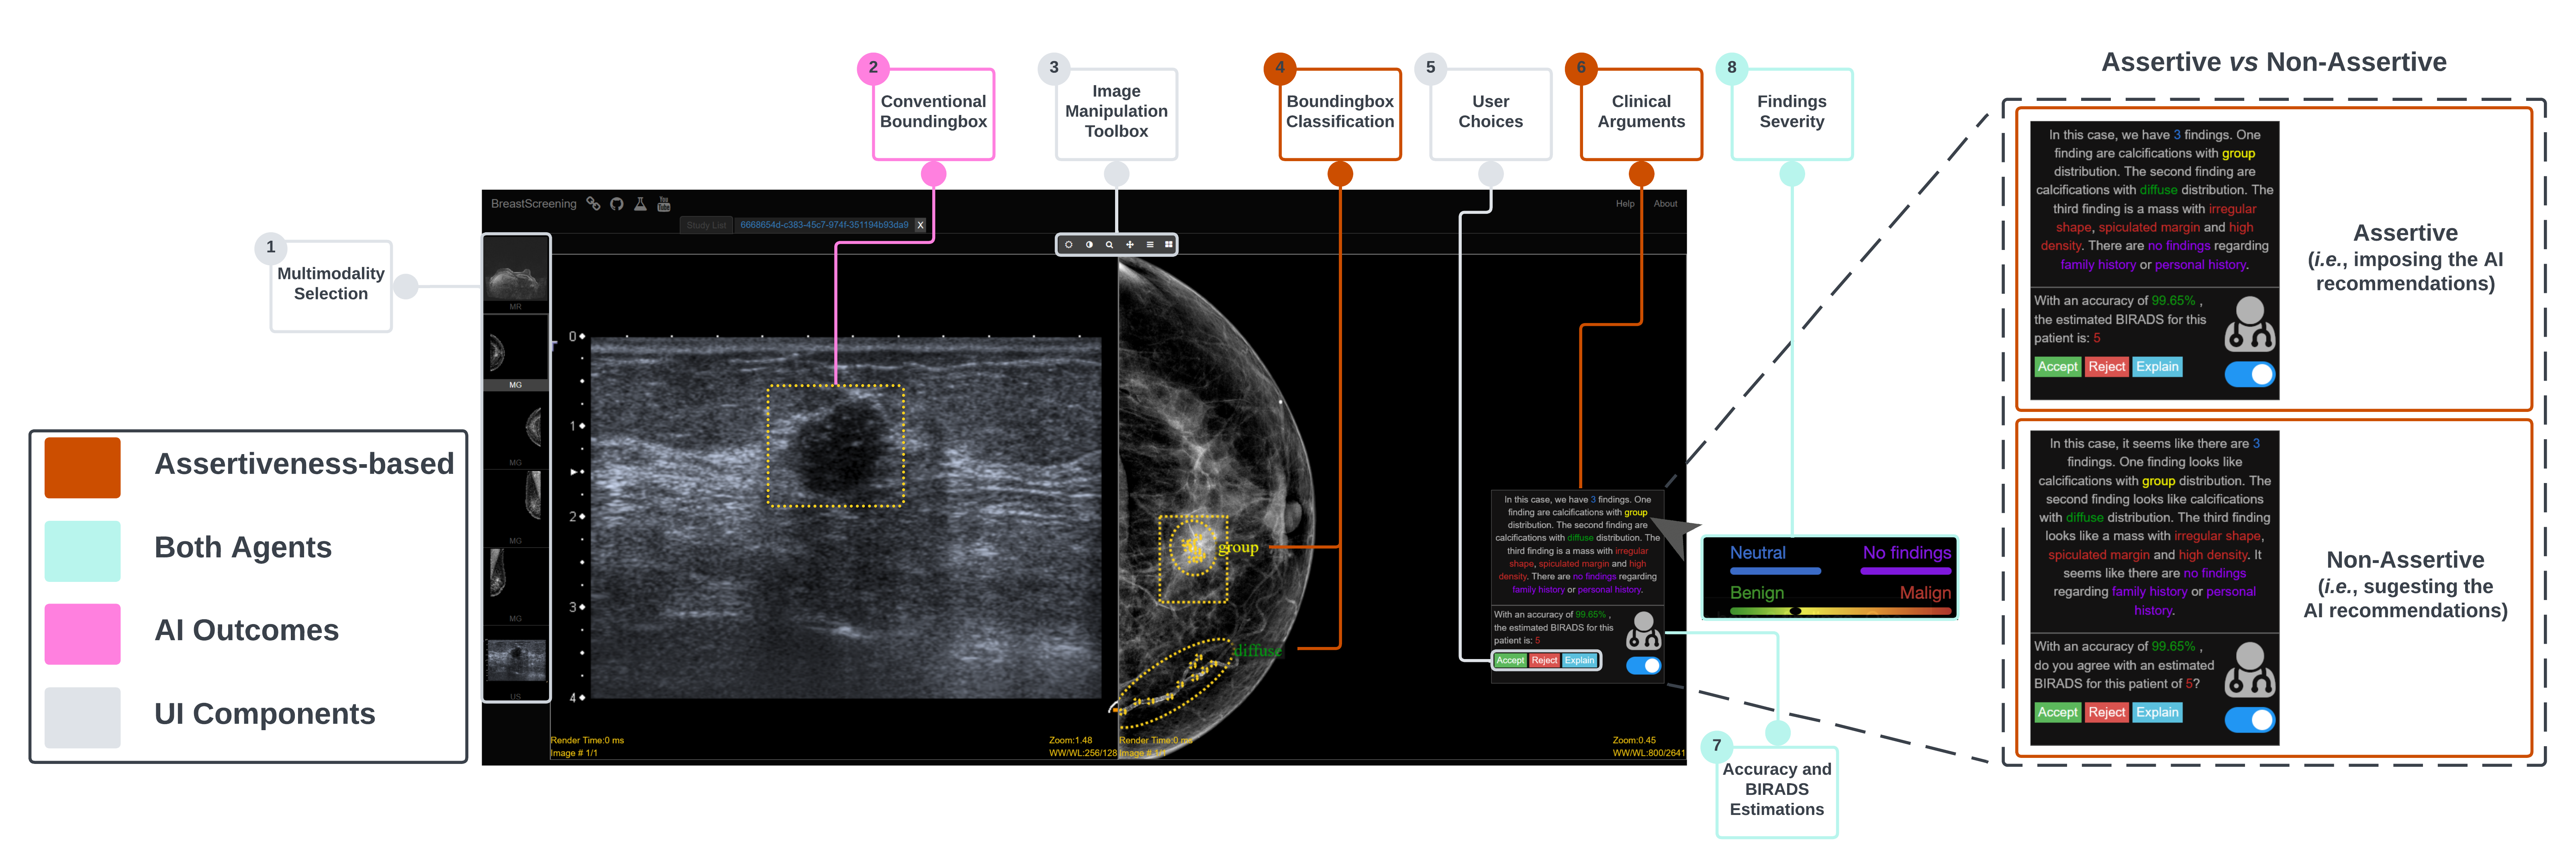
\includegraphics[width=1.000\textwidth]{fig112}
\caption[]{Interface for conventional and assertiveness-based AI agents for medical imaging analysis. Attributes are associated with numbers in each testing condition. When a clinician hovers the mouse over each variable ({\it e.g.}, accuracy, BIRADS, or any other clinical argument of attribute 6), the AI agent will pop up a window to inform the severity of each finding. The colors are ranging from benign (green) to malign (red). The number of findings is displayed in a neutral blue color, reflecting the importance of individual severity rather than quantity. Clinicians use purple to indicate family and personal history variables.}
\label{fig:fig112}
\end{figure}
%%%%%%%%%%%%%%%%%%%%%%%%%%%%%%%%%%%%%%%%%%%%%%%%%%%

In our study, both AI agents were designed to communicate this type of {\it quantitative} confidence in two ways (Figure~\ref{fig:fig098}):
(1) for the conventional condition, clinicians could simply see the suggested numeric representation of the BIRADS and the respective accuracy of the model;
(2) for the assertiveness-based condition, the agent was communicating the clinical arguments along with the communication of the BIRADS and accuracy, but this time by descriptive information.
While our conventional agent employed this baseline numeric representation of confidence, our assertiveness-based agent is communicating the {\it quantitative} confidence based on a descriptive sentence of the clinical arguments.
Specifically, the image view-port was augmented with an additional bounding box or circle ellipse {\bf highlighting the lesion characteristics} that were likely to explain the final BIRADS classification.
Note that these suggestions did not dictate the order in which imaging modalities are presented to clinicians.
Indeed, clinicians can remain to decide freely what modalities and clinical arguments are reviewed first.

%%%%%%%%%%%%%%%%%%%%%%%%%%%%%%%%%%%%%%%%%%%%%%%%%%%
\begin{figure}[htpb]
\begin{center}
\centering
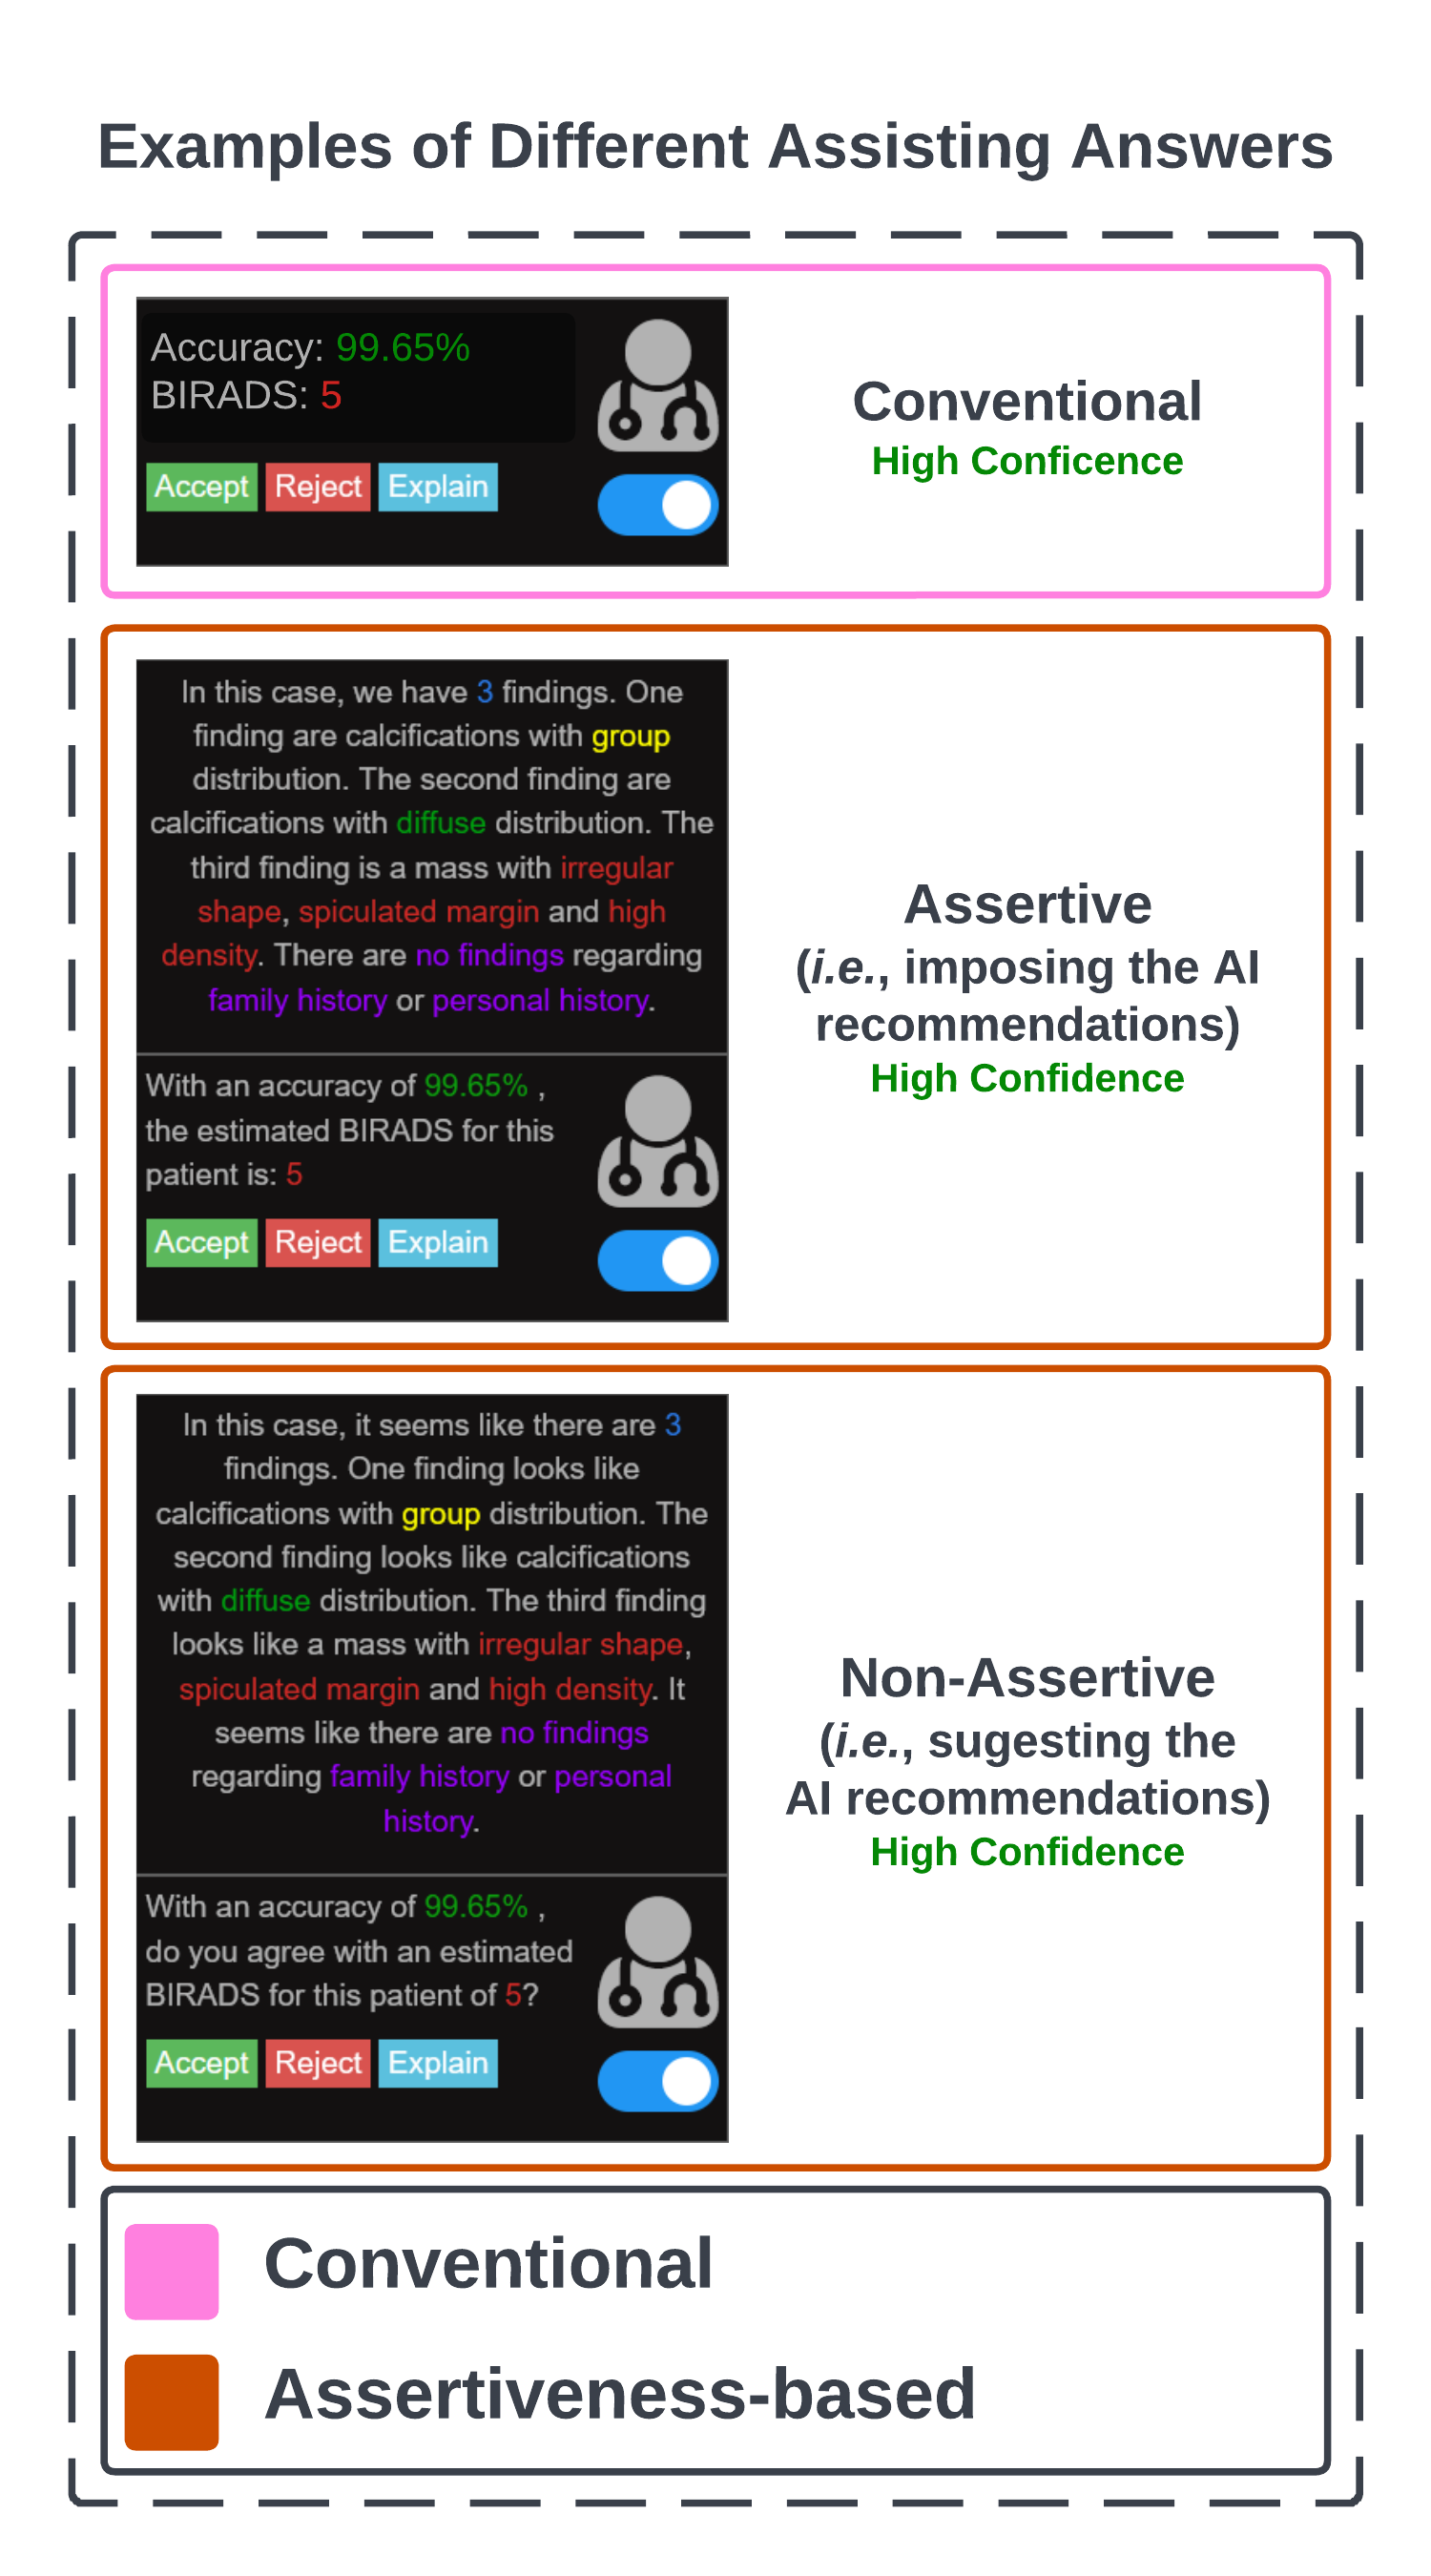
\includegraphics[width=0.625\textwidth]{fig098}
\end{center}
\caption[]{Example of representative use cases for the different testing trials. From top to the bottom, the first agent is representing a conventional example (pink), while the other two are representing assertiveness-based examples (brown), from assertive to non-assertive communication.}
\label{fig:fig098}
\end{figure}
%%%%%%%%%%%%%%%%%%%%%%%%%%%%%%%%%%%%%%%%%%%%%%%%%%%

The patient's detailed augmentation for medical imaging on breast cancer diagnosis was extended with an {\bf assertiveness-based explanation}.
With our system, we are listing human-interpretable clinical arguments for classification and segmentation recommendations that would adapt their communication depending on the personalized and customized demographic characteristics of the clinician.
These clinical arguments corresponded to the classification outputs of an AI model and were trained on data (Section~\ref{sec:chap006005002}) from real-world clinical cases, as described next.

\section{Research Objectives}
\label{sec:app005005}

In this section, we provide a comprehensive overview of our research objectives, which are guided by the research questions and hypotheses outlined earlier (Section~\ref{sec:chap006004} of Chapter~\ref{chap:chap006}).
These research questions and hypotheses serve as a roadmap for our study across the influence of assertiveness-based agents on medical assessments and clinicians' perceptions.
Here, we delve deeper into the specific research questions and hypotheses listed in Section~\ref{sec:chap006004} of Chapter~\ref{chap:chap006}, offering a more detailed perspective on our investigation.
Through this in-depth description, we establish a solid foundation for our investigation, highlighting the key aspects and driving factors that shape our research direction.

Through our research, we aim to contribute to developing effective \ac{AI} systems that align with clinicians' needs and expectations, ultimately enhancing clinical decision-making processes.
While investigating the impact of assertiveness-based agents on medical assessments, we can identify ways to optimize efficiency and accuracy in clinicians' assessments.
Addressing the following research questions and hypotheses with subsequent analysis (Section~\ref{sec:chap006005005} of Chapter~\ref{chap:chap006}) will provide valuable insights that inform the design and implementation of \ac{AI} systems.
Ultimately, these insights will contribute to improving the quality and speed of medical decision-making, benefiting both clinicians and patients.

For {\bf RQ1}, we assume that personalized and customized explanations can inform clinical decision-making.
Therefore, it will increase clinicians' classification accuracy without reducing their time performance over diagnosis.
Primarily, we envision that adapting the communication of personalized explanations is crucial for successfully informing clinicians' decision-making.
For that, we propose three hypotheses about efficiency, accuracy, and the impact on different levels of clinicians' expertise.
Hypothesis {\bf H1.1} suggests that clinicians' efficiency, measured by the time performance per diagnosed patient, will be higher with an assertiveness-based agent.
Hypothesis {\bf H1.2} states that the classification accuracy of clinicians will not be compromised when using an assertiveness-based agent.
Hypothesis {\bf H1.3} suggests that the accuracy differences between novice and expert clinicians will depend on the tone of the personalized explanations provided by the assertiveness-based agent.
By investigating these hypotheses, we aim to shed light on the effectiveness of assertiveness-based agents in informing and supporting clinicians' decision-making processes.

The \ac{HCI} research community has settled that poor user perception can be a barrier to the adoption of technology regardless of performance~\cite{10.1145/3313831.3376506, 10.1145/3479549}.
The user perceptions of preference and trust are essential in predicting technology adoption.
Hence, it is crucial to investigate clinicians' perceptions, as we do in {\bf RQ2}.
Beyond the primary outcome regarding reliability in \ac{AI}-assisted clinical assessments, our goal is also to understand how clinicians perceive assertiveness-based agents.
Because of that, we propose four hypotheses related to clinicians' preference, trust, workload, and perception based on different levels of expertise.
Hypothesis {\bf H2.1} suggests clinicians prefer an assertiveness-based agent.
Hypothesis {\bf H2.2} states that clinicians will consider an assertiveness-based agent more trustworthy.
Hypothesis {\bf H2.3} suggests that personalized highlights and explanations provided by the agent will not increase clinicians' workload or decrease usability.
Finally, Hypothesis {\bf H2.4} proposes that novice and expert clinicians will perceive the reliability and capability of the agent differently, depending on the levels of assertiveness.
By examining these hypotheses, we aim to gain insights into how clinicians perceive and interact with assertiveness-based agents, contributing to the development of effective and user-centered \ac{AI} technologies in healthcare.

Addressing these research questions and hypotheses (Section~\ref{sec:chap006004} of Chapter~\ref{chap:chap006}) will provide valuable insights into the impact of assertiveness-based agents on medical assessments and clinicians' perceptions.
Our goal is to understand the efficiency and accuracy benefits that these agents can offer without compromising clinicians' valuable time in real-world clinical settings.
Moreover, we recognize the significance of clinicians' perceptions in the successful adoption and integration of intelligent agents into clinical practice.
Thus, developing \ac{AI} systems more effectively to support clinicians in their decision-making process and leading to improved clinical outcomes.

\section{Research Methods and Experimental Design}
\label{sec:app005006}

This section provides a comprehensive detail of the research methods and experimental design employed in our study, building upon the summarized methods outlined in Section~\ref{sec:chap006005} of Chapter~\ref{chap:chap006}.
As a way to improve clinical decision-making, the goal of our study is to attain a deeper understanding of personalized and customized mechanisms, exploring how to adapt the communication of agents depending on the medical experience of clinicians.
Our study draws from 52 semi-structured interviews and user testing with clinicians for breast cancer detection via medical imaging diagnosis.
To accomplish this goal, we designed and implemented a rigorous experimental approach.
Our study employed a two-condition study design, using a within-subjects and counterbalanced experiment.
By employing a within-subjects design, we ensured that each participant in our study experienced both conditions under investigation.
Each participating subject was involved in three distinct trials (Figure~\ref{fig:fig098}), allowing us to collect a wealth of diverse and comprehensive data to analyze.

Interviews were conducted from March 2022 to June 2022.
\acp{RQ} were fused from these interviews and observations (Section~\ref{sec:chap006004} of Chapter~\ref{chap:chap006}), thanks to the support of user-centered activities, such as workshops, focus groups, affinity diagramming, data clustering, and prototype co-design, leading us to reported problems.
Participants in these sessions include clinicians from different healthcare institutions, researchers from the \ac{ML} field, and \ac{HCI} researchers.
Before the work commenced, the study was approved by the ethics committee of each clinical institution.
Next, we describe the details of our controlled experiment, including the task, dataset, information on participants, study procedures, and statistical analysis.

\subsection{Task Details}
\label{sec:app005006001}

In Section~\ref{sec:chap006005001} of Chapter~\ref{chap:chap006}, we provided a summarized description of participation tasks.
Across this section, we are providing further study details concerning participation tasks.
We conducted our study in the field of imaging classification on breast cancer, a clinical domain with typically high False-Positive rates to over-diagnose a patient~\cite{KIM2020e138}.
In particular, we compared our conventional and assertiveness-based agents in assisting trained medical personnel in the task of a breast cancer diagnosis.
For the conventional condition, we used the {\it BreastScreening-AI} framework~\cite{CALISTO2022102285} publicly available (\href{https://mida-project.github.io/prototype-multi-modality-assistant/}{git.io/JMjDi}) and built for the development of medical assistants.
Aside from the already available functionalities of this framework, we developed two conditions for testing our hypothesis from a post-hoc analysis concerning how to personalize and customize the \ac{AI} outcomes to clinicians.

We raised several trials, from a more suggestive (non-assertive) to a more assertive tone of the \ac{AI} recommendations, where clinicians with different levels of expertise interacted with both trials and the conventional.
In the end, all clinicians interacted with one conventional, one non-assertive, and one assertive agent.
Each clinician diagnosed three patients with different severities, where the task was to {\it accept} or {\it reject} the \ac{AI} recommendations.
This experimental setup allowed us to examine how clinicians responded to different assertiveness levels and evaluate their decision-making processes.

There are two groups of clinicians with different medical professional experiences:
(a) novice; and
(b) expert.
Patients are divided into three groups of breast severities:
(i) low severity, representing the \ac{BI-RADS} of 1, meaning there are no findings for that patient and both breasts are healthy;
(ii) medium severity, representing the \ac{BI-RADS} of 2 and 3, meaning there are some findings with a higher probability of benign suspicious; and
(iii) high severity, representing the \ac{BI-RADS} of 4 and 5, meaning there are findings with a higher probability of malign suspicion.
Usually, each patient has available three types of modalities ({\it i.e.}, \ac{MG}, \ac{US}, and \ac{MRI}).
For this task, clinicians need to read six imaging views approximately per each patient:
(1) one \acs{CC} left breast;
(2) one \acs{CC} right;
(3) one \acs{MLO} left;
(4) one \acs{MLO} right;
(5) one \acs{US}; and
(6) one \acs{DCE-MRI} volume with between 100 and 200 frames.
Shortly, clinicians participated as readers while assessing each patient regarding the likelihood and location of the malignancy.

During the task of responding to the lesion localization, the reader clinician provides the severity classification of the clinical argument for that suspicious attribute on the image.
For each image, the clinician classifies the patient's final severity assessment via \ac{BI-RADS} classification by default.
Meaning that, although the patient has some clinical arguments ({\it e.g.}, group microcalcifications with diffuse distribution in Figure~\ref{fig:fig098}) pointing to a \ac{BI-RADS} of 2, if there is a suspicious irregular shape mass with spiculated margin, by default the clinician will consider the final \ac{BI-RADS} as a 5.

The task of diagnosing breast cancer involves reading heterogeneous appearances, ranging from obvious masses with spiculated margins to subtle asymmetric or faint microcalcifications~\cite{Sturesdotter2020}.
This leads to difficulties for clinicians in achieving an accurate diagnosis and consistent interpretation of the patient.
Because of that, clinicians apply rules from radiological guidelines to classify breast images based on visually inspecting the patterns on the image~\cite{doi:10.1148/radiol.2020192534}.

The classification of breast cancer via the \ac{BI-RADS} scale lends itself to a task for our study on AI agents in medical imaging assessments.
Not only, is the task a time-consuming and tedious procedure for clinicians, but it also relies on non-trivial classification tasks.
Indeed, the prior medical literature has established that the medical error of clinicians has between 50\% and 30\% chance of being a false-positive and about 10\% chance of being a \ac{FN}.

\subsection{Dataset Details}
\label{sec:app005006002}

In Section~\ref{sec:chap006005002} of Chapter~\ref{chap:chap006}, we summarized the used dataset.
In this section, we detail the used dataset from a total of 338 cases acquired in \acl{HFF} (Section~\ref{sec:app005006003}).
From this set of cases (Section~\ref{sec:app001002}), 289 were classified by the head of radiology.
Each patient has several images concerning four X-ray \ac{MG} (two in \ac{CC} and two \ac{MLO} views), one \ac{US} image to train the DenseNet model, and roughly \acs{DCE-MRI} images in \ac{MRI} to train the ResNet model.
In the \ac{MRI} volumes, we take several image slices per patient, where the lesion is present.
This provides us roughly 2890 images ({\it i.e.}, 289~\texttimes~(4 + 1 + 5)), that are used to train/test the \ac{AI} models.

Traditional image processing and deep learning techniques require extensive pre-processing.
As a matter of fact, it is known that a cleaning dataset is welcome when training a deep neural network~\cite{RIASATIAN2021102032}.
In our study, this stage is of the utmost importance, since the \ac{MG}, \ac{US}, and \ac{MRI} images contain quite different intensities, and the images are of different sizes.
Thus, before introducing the images to the DenseNet and ResNet models, we pre-process the data (Section~\ref{sec:app001006}).
Specifically, we perform data normalization, so that the images have the same intensity, regardless of the modality.

All the images are resized to 224x224 pixels.
The images are normalized by subtracting their mean and dividing by their standard deviation.
The above size is used since the DenseNet model is prepared to receive the input with this format.

\subsection{Participation Details}
\label{sec:app005006003}

In Section~\ref{sec:chap006005003} of Chapter~\ref{chap:chap006}, we provided a summary of the demographic characteristics of our study participants and the clinical institutions involved.
Now, we will provide a more detailed description of the participants and clinical institutions that collaborated with us in this work.
We recruited 52 clinicians who volunteered to participate in our study from a diverse range of clinical environments (Table~\ref{tab:tab015} on Section~\ref{sec:app005011}), including public hospitals, cancer institutes, and private clinics.

\vspace{0.50mm}

\noindent
Our clinicians were recruited through the already established protocols under this study from 11 different clinical institutions:

\vspace{0.05mm}

\begin{enumerate}
\item \href{https://hff.min-saude.pt}{\acf{HFF}};
\item \href{https://www.ipolisboa.min-saude.pt}{\acf{IPOL}};
\item \href{https://www.chln.min-saude.pt}{\acf{HSM}};
\item \href{http://www.ipocoimbra.min-saude.pt}{\acf{IPOC}};
\item \href{http://www.madeiramedicalcenter.pt}{\acf{MMC}};
\item \href{https://www.sams.pt}{\acf{SAMS}};
\item \href{http://www.chbm.min-saude.pt}{\acf{HB}};
\item \href{https://www.chporto.pt}{\acf{HSA}};
\item \href{https://www.fchampalimaud.org/}{\acf{CF}};
\item \href{https://www.chtmad.min-saude.pt/}{\acf{CHTMAD}}; and
\item \href{https://www.chlo.min-saude.pt/}{\acf{CHLO}};
\end{enumerate}

\vspace{0.05mm}

All clinicians and clinical institutions gave prior permission to use their data for research purposes under this study.
From the demographic questionnaires (Appendix~\ref{chap:app006}), 55.77\% of participants are expert clinicians, whereas 34.62\% are seniors having more than 10 years of practical experience, and 21.15\% are middle clinicians having more than 5 years but less than 10 years.
Similarly, 44.23\% of participants are novice clinicians, whereas 32.69\% are juniors after taking the exam, having up to 5 years of clinical experience, and 11.54\% are interns before the medical specialty exam.
Each clinician was exposed to the three trials ({\it i.e.}, conventional, assertive, and non-assertive) in a counter-balanced manner.

\subsection{Procedure Details}
\label{sec:app005006004}

In Section~\ref{sec:chap006005004} of Chapter~\ref{chap:chap006}, we provided a summarized description of the procedure followed in the study.
Across this section, we further detail some procedures.
After providing an informed consent form for participation in the study, each clinician reported information concerning several self-characteristics (Section~\ref{sec:chap006005003} of Chapter~\ref{chap:chap006}).
First, they reported their demographic characteristics.
Second, they reported their professional backgrounds, such as clinical education ({\it i.e.}, radiology, surgery, nurse, technician, etc.), areas of expertise, work sector, and medical experience.
Finally, information about their experience while reading medical imaging data.
Next, clinicians familiarized themselves for about 3 minutes with our user interface and basic functionalities common to both \ac{AI} agents.

At this stage, each participant interacted with the assistant, {\it accepting} or {\it rejecting} the system suggestion in the two different conditions: (a) conventional; and (b) assertiveness-based.
The set of patients provided participants with 289 patients, while all patients must have at least one of the three available modalities.
Each participant open the set of three patients ({\it e.g.}, {\bf P1}, {\bf P2} or {\bf P3}), chosen randomly, and examined it.
As participants interacted with the system, they could utilize a range of functionalities and tools designed to support their diagnostic tasks.
These functionalities enabled clinicians to access relevant information, perform detailed analysis, and make informed decisions.

Clinicians performed the same task of diagnosing three patients twice, once with the conventional agent and another time with the assertiveness-based agent.
For each task, clinicians were asked to read the suggested \ac{AI} recommendations, where the task ends when clinicians {\it accept} or {\it reject} the proposed \ac{BI-RADS}.
Additionally, clinicians could ask for a visual {\it explanation} inside the image during the task.
The \ac{AI} models fully classified the list of patients, and clinicians could revise the explanations (bounding boxes 2 and 4 of Figure~\ref{fig:fig096}) for the crucial regions to consider.

After each task, clinicians completed a brief feedback questionnaire exploring their perception of each \ac{AI} agent.
The questionnaire included scales to measure three dimensions of trust represented by perceived understanding, competence, and thoughtfulness, as well as cognitive workload by using \ac{NASA-TLX}, and usability by using \ac{SUS}.
With these measures, we aimed to understand the perceived diagnostic utility and decision-making support provided by the \ac{AI} agents, and whether clinicians thought they would use the agents in practice.
Upon completing all the tasks, we measure the preferences using conventional or assertiveness-based agents, and the different levels of assertiveness.

Clinicians assessed the reliability, capability, and overall preference of both \ac{AI} agents.
We also examined the levels of assertiveness, comparing the ratings of novice and expert clinicians.
Specifically, we evaluated the reliability and capability of the communication tones used by the assertiveness-based agent, which ranged from more suggestive to more imposing \ac{AI} recommendations.
Clinicians provided their ratings using a 7-point Likert scale.

\subsection{Specified Analysis}
\label{sec:app005006005}

In Section~\ref{sec:chap006005005} of Chapter~\ref{chap:chap006}, we summarized the analysis conducted in this study.
Here, we provide a detailed explanation of the specific analysis conducted in our study.
We delve into the details of our investigation, focusing on research questions, hypotheses, and statistical tests.
Our analysis examines the impact of the assertiveness-based agent on clinicians' efficiency and efficacy in diagnosing patients, as well as their perceptions of both conventional and assertiveness-based agents.
Additionally, we analyze the qualitative methods used to extract insights from clinicians' feedback and comments.

For {\bf RQ1}, we investigated the impact of our assertiveness-based agent on clinicians' efficiency and efficacy in terms of time performance and accuracy in diagnosing patients with the support of the AI-suggested recommendations.
Similar to the literature, we used the one-way \ac{ANOVA} test~\cite{SADEGHI2022105554, 10.1145/3491102.3517791} to compare both AI agents with respect to the following outcome measures per clinician:
(i) the time (in seconds) for diagnosing each patient ({\bf H1.1.}); and
(ii) accuracy rates via false-positives and false-negatives of clinician-provided classifications ({\bf H1.2.}).
For the efficacy differences between novice and expert clinicians during decision-making ({\bf H1.3.}), we used the chi-squared test of independence~\cite{10.1145/3411764.3445464} to assess the relationship between the expertise of clinicians and the assertiveness levels of the agents.
Regarding human-AI accuracy, our dataset has post-biopsy verification, meaning that we could measure the real \ac{GT} of the patient.

For {\bf RQ2}, we compared clinicians' perceptions of both conventional and assertiveness-based agents.
A possible observed pattern in perceived preference ({\bf H2.1.}) and trustworthiness ({\bf H2.2.}) was examined using the \ac{ANOVA} test and statistical significance (p $<$ 0.05) for testing our hypothesis.
Reported scores for cognitive workload and usability ({\bf H2.3.}) were compared between the two AI agents using statistical significance (p $<$ 0.05) for computing the likelihood of confidence.
Last, we used the one-way \ac{ANOVA} test of variance to test the levels of assertiveness for the provided clinical arguments between the two groups ({\it i.e.}, novice and expert clinicians) of medical professional experience.
Specifically, we used this test to measure the perceived preferences of clinicians in terms of reliability and capability ({\bf H2.4.}).
From ``Totally Non-Assertive'' ({\it i.e.}, more suggestive) to ``Totally Assertive'' ({\it i.e.}, imposing \ac{AI} recommendations), we test the overall tendency between novice and expert clinicians of the communication tone.

Finally, we used the open coding comments and feedback from focus groups, workshops, and interviews.
The purpose was to extract emerging themes from open-ended discussions during these sessions~\cite{SHIBUYA2022107131, BIEG2022107249}.
We organized the responses of clinicians using affinity diagrams to cluster workflow clinical practices and main functional ideas of the agents in greater detail~\cite{DEUTSCH2019122, 10.1145/3491101.3519863}.
Moreover, we used affinity diagramming to uncover clinicians' preferences and concerns based on the data gathered in a thematic ({\it e.g.}, card sorting) coding method.
This information was then used to inform our conclusions about exploring how to personalize and customize the AI recommendations by adapting the communication tone.

Clinicians were asked to reflect on how they used to make their decisions, what information they need to be explained by the AI models, and why they need that.
These qualitative analysis methodologies enable the identification of emerging themes in the data for revealing design considerations.
In Section~\ref{sec:chap006006003} of Chapter~\ref{chap:chap006}, recurring themes are reported as we detail them, with provided feedback and comments from these sessions with clinicians.

\section{Detailed Outcomes Investigation}
\label{sec:app005007}

In this section, we provide a detailed investigation of the outcomes obtained from our study.
This section expands upon the summarized results presented in Section~\ref{sec:chap006006} of Chapter~\ref{chap:chap006}, offering a more comprehensive data analysis.
To test our hypotheses, we used the \texttt{scipy} library from \texttt{python} to conduct a one-way \ac{ANOVA} test, with the level of medical professional experience as the main factor on the dependent variables~\cite{CASALE2022107302}.
The alpha level ($\alpha$ = 0.05) was set for statistics, and the effect size was used to quantitatively measure the magnitude of the experimental comparison effect between variables~\cite{Yigit_Mendes_2018, 10.1145/3180155.3182556}.
Briefly, we focus on statistically significant results and selectively report the results to address our hypotheses by following literature recommendations~\cite{10.1145/3301275.3302289, 10.1145/3290605.3300234, 10.1145/3491102.3517791}.
Next, we investigate the time performance (Figure~\ref{fig:fig099}), accuracy (Figure~\ref{fig:fig084}), and decision (Table~\ref{tab:tab014}) rates of clinicians, while addressing their preference choices (Figure~\ref{fig:fig085}), agreement comparisons (Table~\ref{tab:tab013}), reliability and capability (Figure~\ref{fig:fig091}).

%%%%%%%%%%%%%%%%%%%%%%%%%%%%%%%%%%%%%%%%%%%%%%%%%%%
\begin{figure}[htpb]
\centering
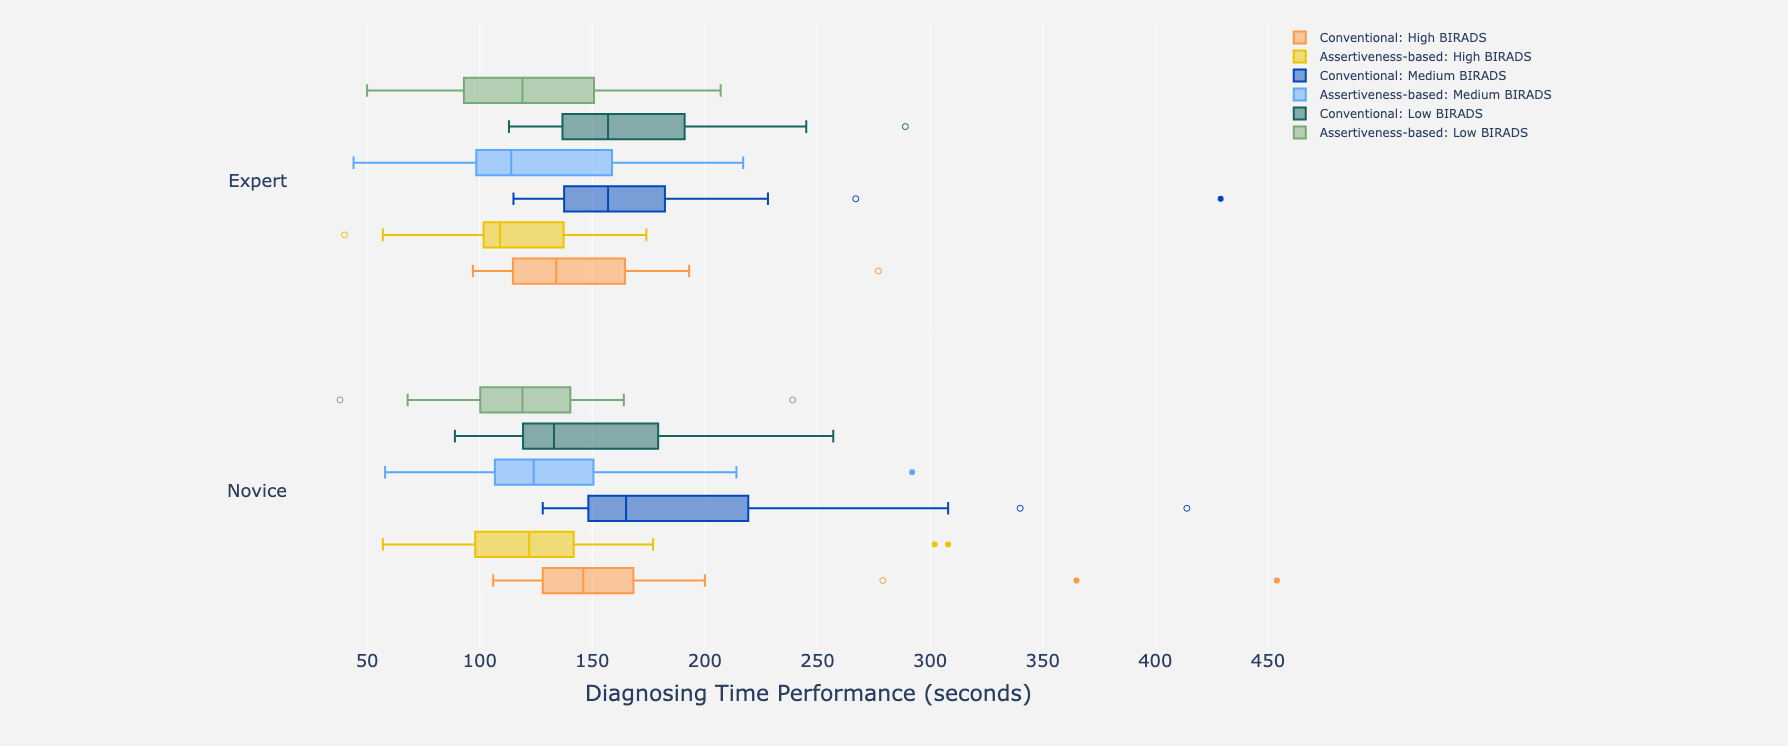
\includegraphics[width=1.000\textwidth]{fig099}
\caption[]{Diagnosing time performance in seconds of novice and expert clinicians to fully diagnose one patient. Different colors are representing different agent trials and breast severities of a patient. Clinicians' task was to read each patient and provide a final BIRADS classification by {\it accepting} or {\it rejecting} the AI recommendations.}
\label{fig:fig099}
\end{figure}
%%%%%%%%%%%%%%%%%%%%%%%%%%%%%%%%%%%%%%%%%%%%%%%%%%%

\subsection{RQ1: Assertiveness-Based Agent Impact on Medical Assessments}
\label{sec:app005007001}

In Section~\ref{sec:chap006006001} of Chapter~\ref{chap:chap006}, we summarized some of our obtained results to answer question {\bf RQ1}.
In this section, we provide detailed results to answer our {\bf RQ1}.
These findings offer insights into how incorporating intelligent agents with assertive communication capabilities can optimize the diagnostic process, potentially leading to improved patient care and outcomes.

We hypothesized that using the assertiveness-based communication between clinicians and an intelligent agent, would alter clinicians' workflow and increase the time performance of clinicians ({\bf H1.1.}) during patient diagnosis.
On average, the time performance of clinicians was significantly improved with the assertiveness-based agent (M = 124.02 seconds, SD = 44.60 seconds) than with the conventional agent (M = 166.12 seconds, SD = 60.42 seconds), confirming our hypothesis (Figure~\ref{fig:fig099}).
This difference was significant (F = 11.32, p = 0.005 $<$ 0.05), indicating a large effect size (r = 0.49).
These findings highlight the positive influence of assertiveness-based communication on clinicians' efficiency and suggest its potential as a valuable tool in the context of patient diagnosis.

%%%%%%%%%%%%%%%%%%%%%%%%%%%%%%%%%%%%%%%%%%%%%%%%%%%
\begin{figure}[htpb]
\centering
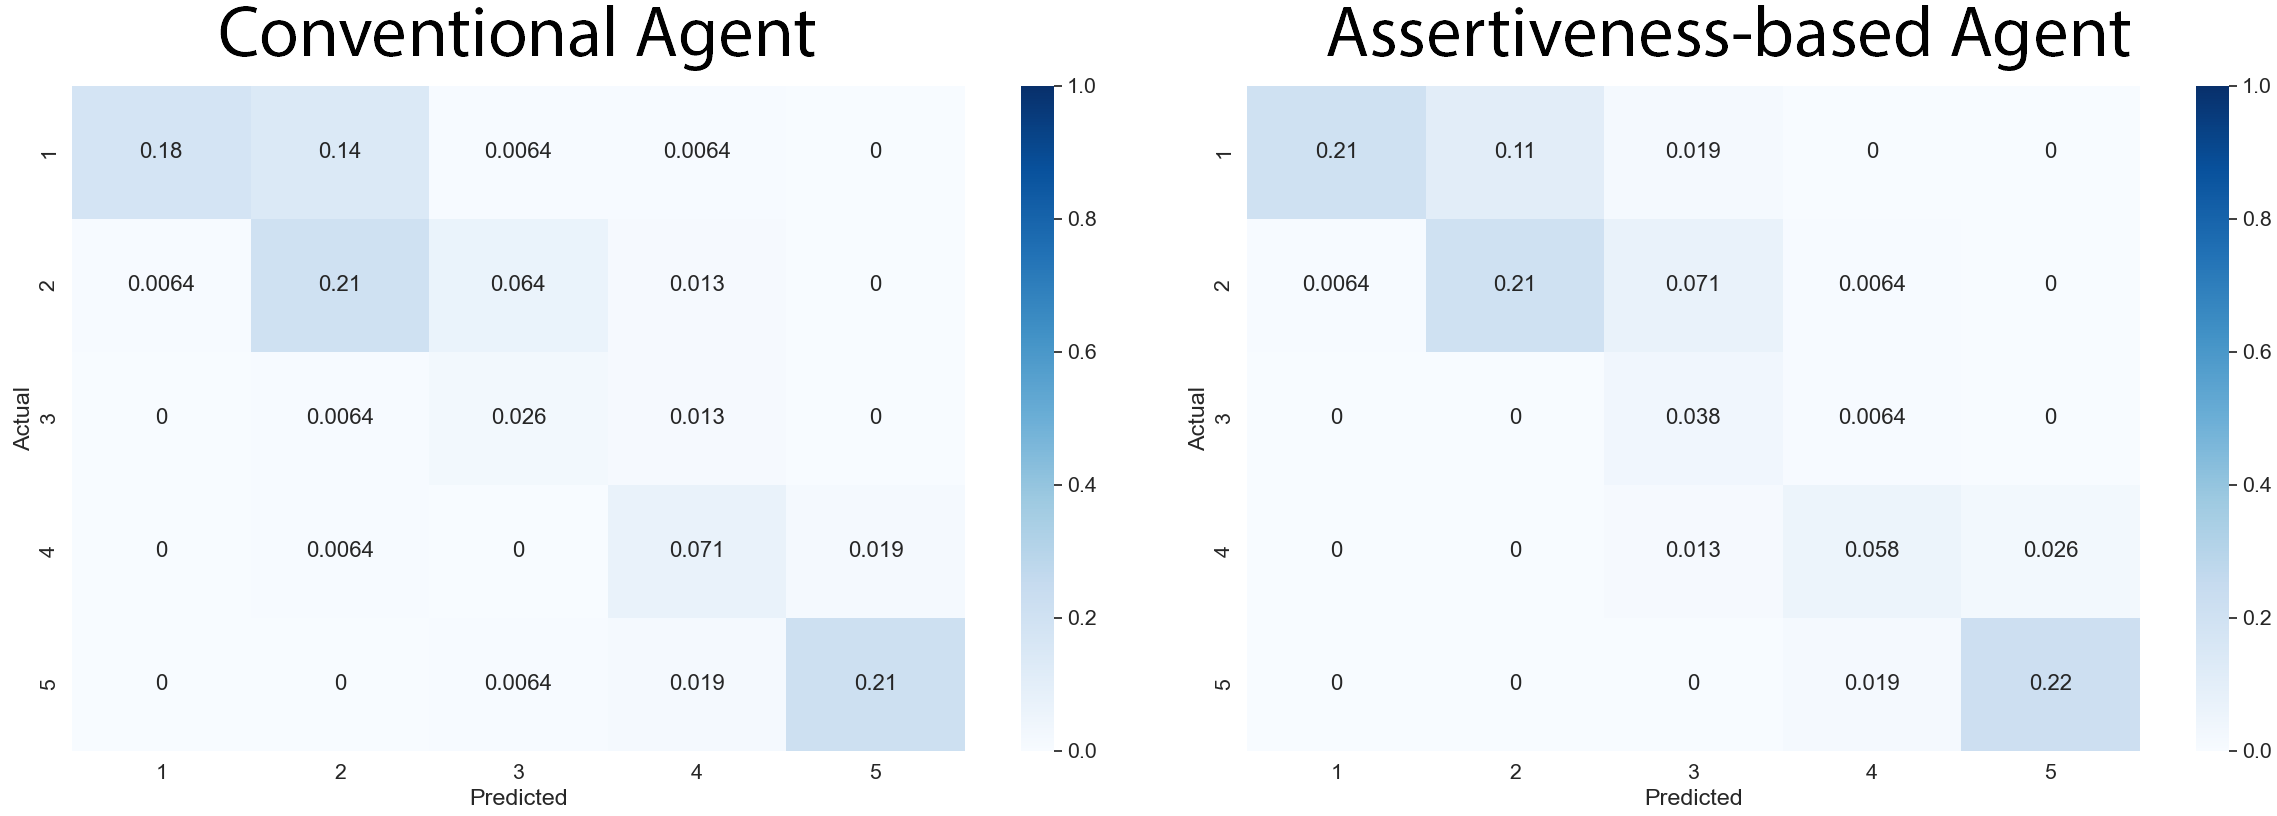
\includegraphics[width=0.855\textwidth]{fig084}
\caption[]{Accuracy rates using a confusion matrix. Comparison between the clinician's BIRADS classification (from 1 to 5) of a patient while using both conventional (left) and assertiveness-based (right) agents. Columns are representing the {\it Predicted} value (collaboration between the clinician and AI), and the rows are representing the {\it Actual} category (biopsy confirmed).}
\label{fig:fig084}
\end{figure}
%%%%%%%%%%%%%%%%%%%%%%%%%%%%%%%%%%%%%%%%%%%%%%%%%%%

In addition to our investigation, we hypothesized ({\bf H1.2}) that using an assertiveness-based agent would not harm clinicians' accuracy.
Our analysis of the results (Figure~\ref{fig:fig084}) revealed no significant difference in accuracy (F = 1.85, p = 0.37 $>$ 0.05).
These findings support our hypothesis, indicating that clinicians' ability to classify patients was not negatively affected by the assertiveness-based explanations.
Consequently, the integration of the assertiveness-based agent into clinical settings can proceed without compromising the accuracy of patient diagnoses.
Moreover, Table~\ref{tab:tab014} presents additional insights into the acceptance and rejection rates of \ac{AI} recommendations by clinicians, further reinforcing our conclusions and demonstrating the robustness of the assertiveness-based approach.
Overall, our study contributes valuable evidence to support the adoption of assertiveness-based agents in medical settings, offering improved workflow and decision-making without compromising diagnostic accuracy.

%%%%%%%%%%%%%%%%%%%%%%%%%%%%%%%%%%%%%%%%%%%%%%%%%%%
% Please add the following required packages to your document preamble:
% \usepackage{multirow}
% \usepackage{graphicx}
% \usepackage[table,xcdraw]{xcolor}
% If you use beamer only pass "xcolor=table" option, i.e. \documentclass[xcolor=table]{beamer}
\begin{table*}[bp]
\resizebox{\textwidth}{!}{%
\begin{tabular}{|c|cc|cc|cc|cc|cc|ll|}
\hline
                                     & \multicolumn{2}{c|}{\textbf{Correct Accepts}}                                        & \multicolumn{2}{c|}{\textbf{Correct Rejects}}                                      & \multicolumn{2}{c|}{\textbf{Overall Corrects}}                                       & \multicolumn{2}{c|}{\textbf{Wrong Accepts}}                                        & \multicolumn{2}{c|}{\textbf{Wrong Rejects}}                                          & \multicolumn{2}{l|}{\textbf{Overall Mistakes}}                                       \\ \cline{2-13} 
\multirow{-2}{*}{\textbf{Trials}} & \multicolumn{1}{c|}{\textbf{Novice}}                & \textbf{Expert}                & \multicolumn{1}{c|}{\textbf{Novice}}               & \textbf{Expert}               & \multicolumn{1}{c|}{\textbf{Novice}}                & \textbf{Expert}                & \multicolumn{1}{c|}{\textbf{Novice}}               & \textbf{Expert}               & \multicolumn{1}{c|}{\textbf{Novice}}                & \textbf{Expert}                & \multicolumn{1}{l|}{\textbf{Novice}}                & \textbf{Expert}                \\ \hline
\textbf{Conventional}                & \multicolumn{1}{c|}{{\color[HTML]{9A0000} 68\%}}    & {\color[HTML]{9A0000} 62\%}    & \multicolumn{1}{c|}{{\color[HTML]{9A0000} 1.7\%}}  & 1.77\%                        & \multicolumn{1}{c|}{{\color[HTML]{9A0000} 69.70\%}} & {\color[HTML]{9A0000} 63.77\%} & \multicolumn{1}{c|}{3.7\%}                         & 4.1\%                         & \multicolumn{1}{c|}{{\color[HTML]{9A0000} 26.6\%}}  & {\color[HTML]{9A0000} 32.13\%} & \multicolumn{1}{l|}{{\color[HTML]{9A0000} 30.30\%}} & {\color[HTML]{9A0000} 36.23\%} \\ \hline
\textbf{Assertive}                   & \multicolumn{1}{c|}{{\color[HTML]{009901} 79.83\%}} & 63.13\%                        & \multicolumn{1}{c|}{1.76\%}                        & {\color[HTML]{009901} 2.63\%} & \multicolumn{1}{c|}{{\color[HTML]{009901} 81.59\%}} & 65.76\%                        & \multicolumn{1}{c|}{{\color[HTML]{009901} 3.05\%}} & {\color[HTML]{9A0000} 4.75\%} & \multicolumn{1}{c|}{{\color[HTML]{009901} 15.36\%}} & {\color[HTML]{009901} 29.49\%} & \multicolumn{1}{l|}{{\color[HTML]{009901} 18.41\%}} & 34.25\%                        \\ \hline
\textbf{Non-Assertive}               & \multicolumn{1}{c|}{72.64\%}                        & {\color[HTML]{009901} 64.72\%} & \multicolumn{1}{c|}{{\color[HTML]{009901} 2.99\%}} & {\color[HTML]{9A0000} 1.69\%} & \multicolumn{1}{c|}{75.63\%}                        & {\color[HTML]{009901} 66.41\%} & \multicolumn{1}{c|}{{\color[HTML]{9A0000} 5.48\%}} & {\color[HTML]{009901} 3.91\%} & \multicolumn{1}{c|}{18.89\%}                        & 29.68\%                        & \multicolumn{1}{l|}{24.37\%}                        & {\color[HTML]{009901} 33.59\%} \\ \hline
\end{tabular}%
}
\caption[]{Frequency of clinicians, showing how often they accept or reject the AI recommendations. These rates show how often clinicians switched to a different conclusion after interacting with each agent. The ``Overall Corrects'' denote the frequency of time clinicians correctly accept (``Correct Accepts'') the recommendations of the AI agents and correctly reject (``Correct Rejects'') by changing the wrong AI recommendation to the right diagnostic. On the other hand, ``Overall Mistakes'' is denoting the frequency of times clinicians wrongly accept (``Wrong Accepts'') the AI recommendations, meaning that the AI agent was wrong, but they accept it, and wrongly reject (``Wrong Rejects''), meaning the AI agent was right, but clinicians changed to the wrong final diagnostic.}
\label{tab:tab014}
\end{table*}
%%%%%%%%%%%%%%%%%%%%%%%%%%%%%%%%%%%%%%%%%%%%%%%%%%%

We further examined the potential impact of personalized explanations by customizing the agent communication differently between the two groups of professional medical experience, {\it i.e.}, novice and expert clinicians ({\bf H1.3.}).
We observed a significant association between the levels of assertiveness ({\it e.g.}, from non-assertive to assertive communication tone of the clinical arguments) and the medical professional experience while revising \ac{AI} recommendations ($\chi^2$ = 3.84, p = 0.001 $<$ 0.05).
In other words, the chance of a patient getting classified correctly by a novice was significantly higher (Accuracy\textsubscript{novice} = 91\%) with the assertive agent ({\it i.e.}, imposing \ac{AI} recommendations) than with the non-assertive ({\it i.e.}, more suggestive \ac{AI} recommendations).
On the contrary, the chance of correctly classifying the patient by an expert clinician was slightly higher (Accuracy\textsubscript{expert} = 78\%) with the non-assertive agent.
The odds of a patient getting classified correctly by a novice had a 17.4\% chance higher with the assertive agent, while expert clinicians had a 4.4\% chance higher with the non-assertive agent.
These findings suggest that the level of assertiveness of the agent's communication may need to be tailored to the experience level of the clinician.
Exploring the communication tone indicates that agents may need to be more assertive for novice clinicians, while a suggestive tone may be more appropriate for expert clinicians.

Finally, Table~\ref{tab:tab014} shows how often clinicians accept or reject the \ac{AI} recommendations, as well as how often they switch to a different conclusion.
The highest overall correct rate was 81.59\% in the assertive trial for novice clinicians and 66.41\% in the non-assertive trial for expert clinicians.
Moreover, experts are switching to fewer wrong decisions with the non-assertive agent (Total = 33.59\%).
On the other hand, novices are switching to less wrong decisions with the assertive agent (Total = 18.41\%).
Overall, clinicians made better decisions with assertiveness-based assistance while exploring how to adapt the communication tone.
The results suggest that the assertiveness-based condition may have been more favorable to both novice and expert clinicians, with higher correct acceptance and correct reject rates compared to the conventional condition.
The results highlight the importance of scenario design in evaluating clinicians' performance, as the trials had a significant impact on the performance of both novice and expert clinicians.

\subsection{RQ2: Assertiveness-Based Agent Perceptions of Clinicians}
\label{sec:app005007002}

In Section~\ref{sec:chap006006002} of Chapter~\ref{chap:chap006}, we presented a summary of our findings on question {\bf RQ2}.
In this section, we delve deeper into the detailed results obtained to address our research question. Our focus for {\bf RQ2} was to investigate clinicians' perceptions of both \ac{AI} agents.
By examining clinicians' feedback and perspectives, we gained valuable insights into their experiences and attitudes toward assertiveness-based and conventional agents.
These insights provide a comprehensive understanding of how clinicians perceive and interact with the \ac{AI} technology in the context of medical assessments.

The results for our hypothesis ({\bf H2.1}) that clinicians would have a preference (Figure~\ref{fig:fig085} on Section~\ref{sec:chap006006002} of Chapter~\ref{chap:chap006}) for an assertiveness-based agent were statistically significant (F = 8.35, p = 0.001 $<$ 0.05) between the groups of interns, juniors, middles, and seniors with a large effect size (r = 0.41).
Out of the 52 participants who expressed a preference, 66\% preferred the assertiveness-based agent, and another 24\% preferred the conventional agent, while 10\% did not have a preference.
These findings highlight the importance of considering clinicians' preferences and the potential benefits of incorporating assertiveness-based communication in medical decision-making processes.

We also examined the perceived trust and understanding of clinicians towards both the conventional and assertiveness-based agents (Table~\ref{tab:tab013}).
The results showed slight differences (F = 19.47, p = 0.06 $>$ 0.05) in overall perceived trust between the two agents, indicating a comparable level of trustworthiness.
There were no significant differences (p = 0.14 $>$ 0.05) in understanding between the agents.
However, the assertiveness-based agent was perceived to have greater competence (p = 0.04 $<$ 0.05), suggesting that it was seen as more capable.
Additionally, clinicians demonstrated higher levels of thoughtfulness with the assertiveness-based agent than with the conventional agent (p = 0.001 $<$ 0.05), indicating a more engaged and attentive response.
These findings partially support our hypothesis ({\bf H2.2.}) regarding trust, understanding, competence, and thoughtfulness.

We also evaluated if there were no significant differences in workload and usability between conventional and assertiveness-based agents.
Specifically, there were no significant differences between the workload scores of the two \ac{AI} agents on \ac{NASA-TLX} (p = 0.38 $>$ 0.05).
Furthermore, we observed no significant differences between the usability scores on \ac{SUS} (p = 0.38 $>$ 0.05).
Hence, providing support for our {\bf H2.3.} hypothesis for workload and usability.

%%%%%%%%%%%%%%%%%%%%%%%%%%%%%%%%%%%%%%%%%%%%%%%%%%%
\begin{table}[htpb]
\resizebox{\textwidth}{!}{%
\begin{tabular}{ccc}
\hline
Questions                                                            & Conventional & Assertiveness-based \\ \hline
Overrall, I can trust in the agent recommendations.                  & 86\%         & 90\%                \\
I understand what the system is thinking.                            & 91\%         & 94\%                \\
The system seems competent.                                          & 82\%         & 92\%                \\
The agent shows great thoughtfulness while dealing with the patient. & 71\%         & 75\%                \\ \hline
\end{tabular}%
}
\caption[]{Comparison for the percentage of agreement between conventional and assertiveness-based agents. The questions are following the three {\it dimensions of trust} represented by perceived {\it understanding}; {\it competence}; and {\it thoughtfulness}.}
\label{tab:tab013}
\end{table}
%%%%%%%%%%%%%%%%%%%%%%%%%%%%%%%%%%%%%%%%%%%%%%%%%%%

Finally, to assess how clinicians perceive the levels of assertiveness differently (Figure~\ref{fig:fig091}), we compared the preferences in terms of reliability and capability from non-assertive (suggestive) to assertive (authoritative) communication of the clinical arguments.
Here, we can denote that there are significant differences in reliability (F = 31.36, p = 0.0001 $<$ 0.05) and capability (F = 18.17, p = 0.0003 $<$ 0.05) between groups of novice and expert clinicians.
Novice clinicians perceived assertive communication as more reliable (61\%), although not mainly feeling the same for capability (48\%).
On the other hand, expert clinicians perceived non-assertive communication as more reliable (69\%) and capable (66\%).
Therefore, we can observe that the {\bf H2.4.} hypothesis is supported by showing that novice and expert clinicians will perceive differently the provided clinical arguments depending on if the agent is imposing the \ac{AI} recommendations or being more suggestive.

%%%%%%%%%%%%%%%%%%%%%%%%%%%%%%%%%%%%%%%%%%%%%%%%%%%
\begin{figure}[htpb]
\centering
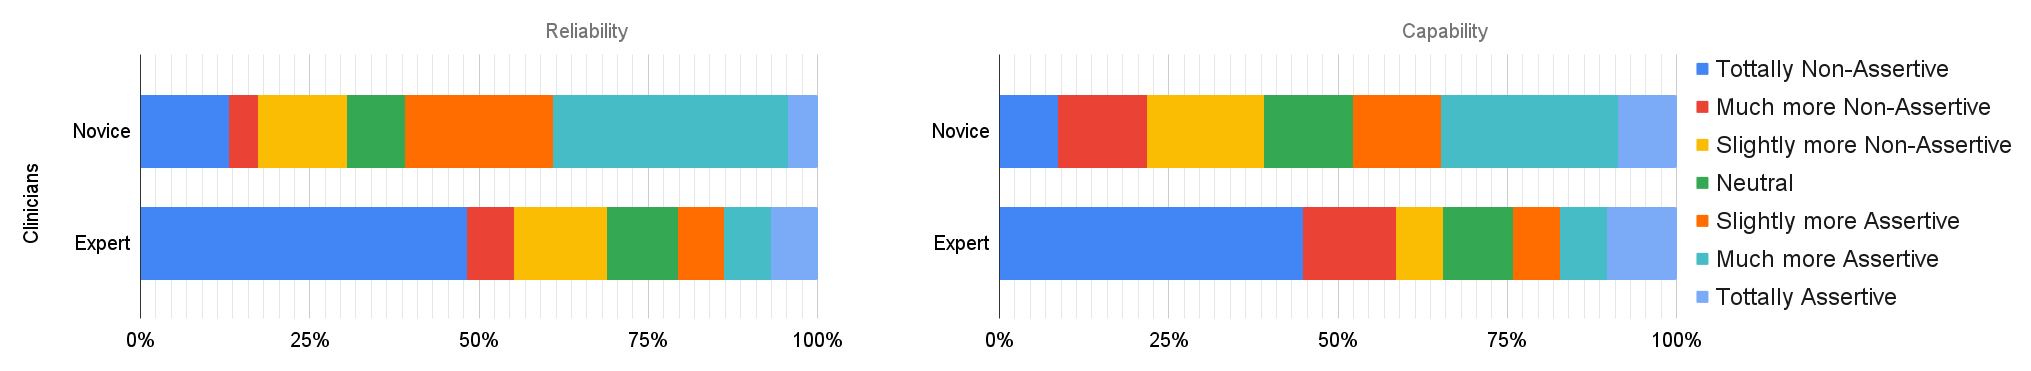
\includegraphics[width=1.000\textwidth]{fig091}
\caption[]{Ratings between novice and expert clinicians for perceived reliability and capability. Clinicians rated each agent, ranging from {\it Totally Non-Assertive} to {\it Totally Assertive} communication.}
\label{fig:fig091}
\end{figure}
%%%%%%%%%%%%%%%%%%%%%%%%%%%%%%%%%%%%%%%%%%%%%%%%%%%

\subsection{Qualitative Insights}
\label{sec:app005007003}

Following a similar approach described in Section~\ref{sec:chap005005004002} of Chapter~\ref{chap:chap005}, we adopted a participatory approach for qualitatively analyzing our study results.
Given our collected data (focus group sessions, participant opinions, and transcripts), we used emergent affinity diagrams to identify common themes in how participants intend to have their clinical arguments and visualize the \ac{AI} recommendations.
Our qualitative analysis of participant responses to open-ended survey questions yielded insights on how assertiveness-based agents can affect clinicians’ workflows and their mental models.
This section further details what was summarized in Section~\ref{sec:chap006006003} of Chapter~\ref{chap:chap006}.

\subsubsection{Altering Clinical Workflows}
\label{sec:app005007003001}

To validate the proposed design, we discussed with clinicians how could they use these set of personalized agent communications to perform diagnosis on a real clinical environment.
The goal is to understand whether an assertiveness-based agent can (a) be compatible integrated into clinicians' workflow, and (b) provide added values to clinicians' diagnosis process.
Next, we summarize the main opinions of clinicians between conventional and assertiveness-based assistance, as well as between suggestive (non-assertive) and more imposing (assertive) AI recommendations.

One major criticism to the traditional approach of representing the AI recommendations with numeric BIRADS classification, accuracy of the output and heatmap values is that it is not sufficient for clinicians to make sense of the decision-making reasoning behind the output classifications.
In particular, when the output accuracy is lower than 80\% confidence.
Our qualitative findings suggest that in choosing between numeric representations of the AI output classifications and human-interpretable arguments while exploring how to adapt the communication, clinicians found the latter to be more effective during decision-making.
This highlights the necessity for AI systems to be designed with a user-centered approach~\cite{10.1145/3491102.3517789}, taking into account the preferences and needs of the end-users (in this case, clinicians) to ensure that they are usable and effective in real-world scenarios.

\vspace{2.5mm}

\noindent
Specifically, a middle clinician ({\it i.e.}, expert clinician) reported:

\vspace{2.5mm}

\noindent
``{\it When I was interacting with the AI agents, the first thing I did was to find classification conflicts between the final BIRADS of the patient, the BIRADS of each image, output accuracy, and clinical arguments. Something that I couldn't do so well in the first [conventional] agent, but could do better for the second [assertiveness-based] one.}'' (C51)

\vspace{2.5mm}

In domains where clinicians' availability is rare, it can be exceedingly hard to obtain an immediate second reader every time a clinician needs the opinion of another human expert.
Clinicians shared a positive attitude towards the use of an assertiveness-based agent to aid their decision-making, since we are exploring how these set of agents are adapting the communication depending on the level of professional medical experience.
Something that is common when a senior (assertively) talks to an intern, while our agent is mimicking the same communication conditions.
Such mimicking behavior must be designed to help diagnosis without incurring in learning misinformation that interrupts the main clinical workflow.

\noindent
Here, a senior clinician ({\it i.e.}, expert clinician) is sustaining the above argument by reporting that:

\vspace{2.5mm}

\noindent
``{\it Adapting the communication between more suggestive [non-assertive] or assertive tone of the clinical arguments can help the diagnosis workflow. I may prefer a suggestive agent, but an assertive agent will be more helpful for my interns concerning an educational purpose.}'' (C15)

\vspace{2.5mm}

Categorically, clinicians were mostly stating that they could understand how such personalized communication could be beneficial to customize the interaction between humans and AI.
In particular, clinicians valued the opportunity to choose the communication tone to explore the clinical arguments in a more detailed fashion.
Our qualitative findings suggest that most clinicians (48/52) found the assertiveness-based agent to be more helpful and reliable.
These findings also support our claim that customization could have a positive impact on the decision-making process and improve the overall effectiveness of AI-assisted systems.

\vspace{2.5mm}

\noindent
As another example, a junior clinician ({\it i.e.}, novice clinician) reported that:

\vspace{2.5mm}

\noindent
``{\it When the agent is talking to me in a more assertive way, I can feel more safe of my decision... and feeling more assurance of the right answer.}'' (C17)

\vspace{2.5mm}

This analysis further highlights the effectiveness of the assertiveness-based agent in personalizing and customizing the communication of the agent, taking into account differences of medical professional experience.
That is, 37 out of 52 clinicians in our study explicitly mentioned that their workflow differed between the two agents.
Particularly, clinicians showed different confidence and trusting opinions depending on the levels of assertiveness.

\vspace{2.5mm}

\noindent
For instance, an intern clinician ({\it i.e.}, novice clinician) reported that:

\vspace{2.5mm}

\noindent
``{\it It seems like, when I was interacting with the more suggestive [non-assertive] assistant, it has the same doubts on the communication tone as I am. The more assertive assistant gave me higher confidence in the decision.}'' (C10)

\vspace{2.5mm}

\noindent
On the other hand, a senior clinician ({\it i.e.}, expert clinician) reported the following:

\vspace{2.5mm}

\noindent
``{\it In my opinion, I don't like the communication tone and the way assertive agents are reporting the clinical arguments. Imposing the AI recommendations feels like I need to follow the orders they give to me. I prefer a more suggestive agent, asking me if the clinical arguments are well classified or not.}'' (C49)

\vspace{2.5mm}

To conclude, these levels of personalizing and customizing the agent communication ({\it e.g.}, from less assertive to more assertive) are important to take into account when designing systems for critical domains.
Especially, for decision-making under these clinical workflows.
We found that assertiveness-based not only enhanced decision-making, but also helped clinicians to develop a mental model of the AI agents, or probe for the likelihood of the diagnosis.
Next, we describe in what manner our work is leveraging these insights.

\subsubsection{Agent Mental Models}
\label{sec:app005007003002}

This section examines how clinicians develop mental models of assertiveness-based agents, with expert clinicians using communication tones to anticipate \ac{AI} mistakes and novice clinicians focusing on the learning process.
Effective communication and personalized approaches are crucial for designing intelligent agents that cater to the perspectives of both groups.
Additionally, clinicians form comparative mental models when comparing conventional and assertiveness-based agents, highlighting the importance of effective communication.
These insights inform the design of intelligent agents that offer personalized communication, catering to the perspectives of both novice and expert clinicians while adjusting the levels of assertiveness.

Both novice and expert clinicians have preconceived mental models about the levels of assertiveness in different ways.
As an example, expert clinicians used the output results to disambiguate AI errors from their own errors, depending on the communication tone.
It is, therefore, possible that this reasoning behavior is projected onto the AI agent to anticipate where the agent would likely make mistakes: ``{\it It could be also important to adapt the communication tone of the clinical arguments depending on the AI confidence.}''
From here, we could understand that expert clinicians expect that the assertiveness of a clinical argument can also be adapted depending on the accuracy of the AI output results for that particular variable.
On the contrary, novice clinicians were more focused on the learning process and patient comparisons for educational purposes: ``{\it For me, the most important thing was to look at the provided arguments and understand if they are right from what I learn or from similar cases. A junior like me must know how the machine is thinking to follow the same reasoning process from my side mentally.}''
Hence, it is vital to provide a more `{\it storytelling-like}' view of the patient for novice clinicians, even in a more assertive fashion.

Apart from preconceptions, we further observed that clinicians developed comparative mental models between conventional and assertiveness-based agents: ``{\it The first AI [assertiveness-based] was outstanding… but in the second AI [conventional] I was frustrated with the lack of communication in comparison to the first one.}''
Moreover, the interaction experience of clinicians with the different AI agents can also shape their reasoning while looking for AI recommendation mistakes: ``{\it In the second assistant [assertiveness-based], I look for classification conflicts between the final BIRADS and the clinical arguments, while I couldn't do the same for the first assistant [conventional], taking me more time to see if there are some mistakes.}''

Our intelligent agents can leverage these insights by not only providing personalized and customized communication with different perspectives between novice and expert clinicians, but also correcting behavior while adjusting internal representations of specific levels of assertiveness. Yet, without hurting the time performance of the diagnostic (Section~\ref{sec:chap006006001} of Chapter~\ref{chap:chap006}), nor increasing the workload (Section~\ref{sec:chap006006002} of Chapter~\ref{chap:chap006}).
In sum, these observations support growing evidence that considering the communication of the \ac{AI} outputs ({\it e.g.}, structure, order, and tone of the arguments) can alter the clinicians' perceptions of the mental models of assisting agents.

\section{Insights and Recommendations}
\label{sec:app005008}

In Section~\ref{sec:chap006007} of Chapter~\ref{chap:chap006}, we discussed the impact of personalized communication from assertiveness-based agents on clinicians' decision-making in medical imaging diagnosis.
This section explored the influence of such communication strategies on clinicians' decision-making.
In the upcoming sections, we will analyze insights and provide recommendations for designing intelligent agents in medical imaging.

Overall, the classification accuracy remained unaffected by the incorporation of assertiveness-based communication.
However, our study revealed a significant impact of the explanation tone on the decision-making behavior of novice and expert clinicians.
This finding underscores the importance of developing compliant agents that can offer personalized and tailored explanations to better cater to the specific needs of clinicians.
These future directions in agent development and validation aim to enhance the provision of relevant and customized explanations, further improving the effectiveness of intelligent agents in medical imaging diagnosis.

Participants were keener on following \ac{AI} recommendations that adapt their communication tone than the ones that did not.
Although this effect may occur because of adding more explanations, it is reflected in differences in behavioral decisions between novice and expert clinicians.
We gain even more insight into the effect of tone from the feedback provided by the clinicians across our qualitative analysis.
Our qualitative results show that participants appreciate the idea of adapting tone to probe the likelihood of the diagnosis.
This finding might be in line with the previous research in psychology and decision support science~\cite{Seidel2021}, bringing new directions for the theoretical application of assertiveness-based communication in deep learning systems and clinical domains.

We studied how personalizing and customizing the \ac{AI} recommendations according to the professional experience of each clinician can reduce medical errors and increase satisfaction.
Specifically, we found significant differences in accuracy, perceived reliability, and capability between novice and expert clinicians, depending on the tone of the personalized explanations.
This finding is relevant in designing \ac{AI} agents for the healthcare sector, while contributing to the \ac{HCI} field.

Clinicians' overall preferences and perceived trust were also increased for the assertiveness-based agent compared to the conventional.
Results suggest a significantly higher perceived understanding of the assertiveness-based agent than the conventional variant.
At the same time, the assertiveness-based agent showed to be perceived by clinicians as more competent and thoughtful.
However, our results indicate the existence of other latent variables.
For instance, the demographic characteristics of clinicians with different levels of clinical experience could shape the implementation of intelligent agents to consider the differences in clinicians' perception of \ac{AI} systems generally.

Regarding the results' significance for the \ac{HCI} community, our research focuses on the use of intelligent agents in medical imaging, which is an important and growing area within \ac{HCI}.
By developing personalized and customized explanations, we aim to improve the effectiveness of decision-making by human clinicians, which is a key concern in \ac{HCI}.
Our specific contribution to the \ac{HCI} community is designing a novel interactive approach for personalized and customized explanations of intelligent agents, underpinned by computational principles.
Our approach combines \ac{ML} with image processing techniques to generate explanations tailored to the individual clinician's expertise.
To our knowledge, this is the first time that this approach has been proposed and evaluated in the context of medical imaging.

Concerning the broader implications of our work, we believe it has relevance for both decision-support research and \ac{AI} communication research.
Our approach to personalized and customized explanations has the potential to improve the accuracy and effectiveness of decision-making by humans in critical domains, which is an essential goal in decision-support research.
At the same time, our work contributes to the growing body of research on improving the communication between \ac{AI} systems and human users, a key concern in \ac{AI} communication research.
Next, we are discussing the design implications and generalizability of our findings, by concluding the limitations of our study and directions for future work.

\subsection{Design Considerations}
\label{sec:app005008001}

This section provides more detailed insights and recommendations based on the design implications summarized in Section~\ref{sec:chap006007001} of Chapter~\ref{chap:chap006}.
Our findings have different stages of design implications for the development of novel \ac{AI}-assisted systems in this clinical domain.
Presented findings range from the combination of different knowledge classifiers of the clinical arguments, training these models with enriched information, to the design of user interfaces for embedded intelligent agents.
In addition, it is essential to conduct further research to explore the potential benefits and limitations of different knowledge representation methods and to evaluate the effectiveness of different design features in enhancing the performance of \ac{AI} systems.
Ultimately, our findings aim to inform the development of more human-centered medical \ac{AI} systems that effectively support clinical decision-making and enhance patient outcomes.
As follows, we will provide our recommendations to inform future work on human-centered medical \ac{AI} systems.

\subsubsection{Different Knowledge Combination}
\label{sec:app005008001001}

Building upon the design implications outlined in Section~\ref{sec:chap006007001} of Chapter~\ref{chap:chap006}, this section provides in-depth insights into incorporating granular patient information from model classifiers.
In a real clinical workflow, extra patient information is necessary for a proper breast cancer diagnosis.
Providing the lesion details and relevance of the classification is an important functionality for better decision-making.
From our interviews, we learn that such information is crucial for diagnostic speed and accuracy, as it informs the clinician on what to look for and where to find the lesions.
To better match the \ac{AI} with the mental model of clinicians and provide better guidance, as well as explanations, we should incorporate granular patient information from the model classifiers~\cite{doi:10.1148/ryai.210299}.
For instance, the \ac{AI} might use different classifiers to provide information on the lesion contours, whereas other classifiers are focused on the lesion margins.
This assumption takes us to another recommendation, how should we train the models with such mixed information, for proper integration into real clinical workflows.

Insights and recommendations in this section guide the design and implementation of intelligent agents in medical imaging by incorporating granular patient information from classifiers.
This enhances clinicians' decision-making and emphasizes the need to align the \ac{AI} system with their mental model for personalized guidance.
Future research should explore training models with mixed information to integrate them effectively into clinical workflows.
These considerations foster human-centered and efficient medical \ac{AI} systems, improving clinical outcomes and patient care.

\subsubsection{Training Mixed Models}
\label{sec:app005008001002}

Expanding on the design implications presented in Section~\ref{sec:chap006007001} of Chapter~\ref{chap:chap006}, this section delves into the training of mixed models.
Our study suggests that clinical workflows and trust can be positively affected by endowing personalization of agent communication.
In fact, with the ability to, not only incorporate granular patient information from the mixed model classifiers, but also adapt the tone depending on the medical experience of the clinician.
Implementing such intelligent agents would require that \ac{DL} models are equipped with the additional prediction of mixed clinical arguments ({\it e.g.}, lesion contours, margin, or cancer type of the patient) beyond diagnosis alone.
This additional granular information about the patient could include its importance to the diagnostic, while also customizing the communication tone depending on the various demographic characteristics of clinicians.
Such an idea could be integrated either into one fused training, or by developing multi separated models, one for each clinical variable.

Personalizing agent communication and incorporating granular patient information from mixed classifiers enhances intelligent agents' effectiveness in medical imaging.
To achieve this, deep learning models must predict mixed clinical arguments, such as lesion contours, margins, or cancer type, and adapt communication based on clinicians' experience and demographics.
Fused training or separate models for each variable may be necessary.
These recommendations advance context-aware medical \ac{AI} systems, improving decision-making and benefiting patient outcomes.

\subsubsection{Adapting Communication}
\label{sec:app005008001003}

This section examines personalized communication between agents and clinicians, expanding on the insights summarized in Section~\ref{sec:chap006007001} of Chapter~\ref{chap:chap006}.
In this work, we evaluate one specific way of personalizing and customizing the communication between agents and clinicians with different levels of medical experience.
We did that by exploring how to adapt the communication tone depending on if the agent was communicating with a novice or an expert clinician.
While our results suggest that this communication technique may be effective, we recommend that future work may explore different demographic characteristics of clinicians.
For example, from different medical institutions ({\it e.g.}, public hospitals, private clinics, cancer centers, etc), or different medical fields ({\it e.g.}, family physicians, breast surgeons, etc.), where some behavioral decision-making of clinicians should differ.

Our qualitative results (Section~\ref{sec:chap006006003} of Chapter~\ref{chap:chap006}) show that clinicians are also willing to adapt the communication tone of the clinical arguments depending on the \ac{AI} confidence.
For instance, if confidence is greater than 80\%, then the system should display an Assertive recommendation (Figure~\ref{fig:fig098}, middle).
Otherwise, it should display a Non-Assertive recommendation (Figure~\ref{fig:fig098}, bottom).
As a research direction, we should explore how different performance actions of the intelligent agents will impact the behavioral decision-making of clinicians.

In conclusion, this section explores personalized communication between agents and clinicians, expanding on insights from Section~\ref{sec:chap006007001} of Chapter~\ref{chap:chap006}.
Adapting communication tones based on clinicians' experience shows promise.
Future research should explore demographic characteristics to enhance decision-making.
Qualitative findings indicate clinicians' willingness to adjust communication tone based on \ac{AI} confidence, a warranting investigation into performance impact.
These research directions advance personalized and context-aware communication in medical \ac{AI}, improving care outcomes.

\subsubsection{Generalizability}
\label{sec:app005008001004}

Building upon the insights in Section~\ref{sec:chap006007001} of Chapter~\ref{chap:chap006}, this section explores the generalizability of intelligent agents.
Our study sheds light on using assertiveness-based agents in breast cancer diagnosis through medical imaging.
Caution should be exercised when generalizing the results to other medical domains.
However, similar personalized and customized communication techniques may benefit various medical diagnoses, as the shared challenges across different specialties motivate our study.

Despite our focus on the breast cancer domain, this demographic characteristics of clinicians ({\it i.e.}, differences in behavioral decision-making between novice and expert) is transversal to other applications~\cite{STAHNKE2021103243, LANDRO2020102897, doi:10.1080/21642850.2020.1741372}.
Such claim is making our approach useful beyond the specific domain of breast cancer diagnosis.
For instance, lung cancer diagnosis requires that specialized radiologists visually inspect chest imaging data similar in nature to that used in our study~\cite{10.1145/3313831.3376807}.
In both of these fields, it may be valuable to personalize and customize the agent communication, depending on their background and expertise, leading to more accurate diagnoses and improved patient outcomes.

The potential of personalizing and customizing the agent communication depending on the levels of medical experience can also be addressed for other clinical domains.
As another example, in skin cancer some works are trying to mimic the medical procedures, where clinicians rely on their past experience across similar cases to reach the final diagnosis~\cite{10.1007/978-3-030-87199-4_52, Tschandl2020, Esteva2017}.
Depending on the past experience of that clinician, the agent should adapt the provided information and communication to them, or other customizable techniques.
Others are stating that AI-based systems must be improved with personalized medicine supporting diagnosis and treatment guidance~\cite{Sollini2020, Aerts2016}.
These studies suggest that the recommendations we make for medical imaging diagnosis in this work have been considered independently and may be of merit beyond the development of assertiveness-based agents.

\subsection{Study Constraints}
\label{sec:app005008002}

This section provides a more detailed analysis of the study constraints summarized in Section~\ref{sec:chap006007002} of Chapter~\ref{chap:chap006}.
In this work, we conducted a within-subject experiment to investigate the use of assertiveness-based agents by clinicians in the particular medical domain of breast cancer diagnosis.
We investigate this question through the design and study of Assertiveness-based BreastScreening-AI~\cite{10.1145/3544548.3580682}.
More specifically, this tool was used to explore how an intelligent agent should adapt its communication tone depending on the professional experience ({\it i.e.}, novice vs expert) of the clinician.

Due to the short availability of clinicians and the remote nature of our study, it was challenging to control the tasks of each step in the experiment precisely.
For example, participants varied how long they completed the task for the first patient, in comparison to the second and third patients.
This lack of experimental control may have impacted the degree to which exposure to the first patient, while interacting for the first time with the assertiveness-based agent, affected how clinicians interacted with the latter.
These challenges highlight the importance of future studies with more controlled experimental conditions to validate further and generalize the findings.

Another limitation is related to the implications of liability when using \ac{AI} in medical settings~\cite{10.1145/3555157}, where the legal framework for addressing these issues is still evolving.
The use of \ac{AI} in medical settings raises complex questions that are not yet fully understood or addressed by existing laws and regulations~\cite{10.1145/3411764.3445432}.
This can make it difficult to determine who might be liable in the event of an error or harm caused by an \ac{AI} system.
\ac{AI} systems often operate in complex and dynamic environments, making it challenging to identify the specific factors that led to a particular outcome.
Overall, the limitations concerning the implications of liability when using \ac{AI} in medical settings highlight the need for further research and legal developments in this area.
Policymakers and other stakeholders need to continue to explore these issues and work to address them in a way that ensures the safe and effective use of \ac{AI} in medical settings~\cite{10.1145/3544549.3573827}.
Future efforts should focus on developing robust frameworks and guidelines to mitigate potential risks and establish accountability in deploying \ac{AI} systems in healthcare~\cite{10.1145/3544548.3581393}.

In our study, the assertiveness-based agent was using specific \ac{AI} outputs, curated and selected by us, alongside choosing the most typical clinical setups in a real-world environment.
While prior work has demonstrated the potential of predicting the likelihood of a clinician to trust an \ac{AI} recommendation from raw medical data~\cite{pmlr-v97-raghu19a}, future work should focus on training \ac{DL} models based on personalized and customized explanations to provide human-interpretable arguments for clinicians.

As another future direction to address, we will study the effects of the two different main features of the assertiveness-based agent ({\it i.e.}, explanations and tone), in more conditions separately (Section~\ref{sec:app001007}).
However, inferring useful information for adapting the \ac{DL} model, presents new technical challenges for the \ac{AI} community.
For the \ac{HCI} community, the challenge is making such inferences transparent, considering some behavioral characteristics of clinicians.

\section{Severity Classification}
\label{sec:app005009}

\ac{BI-RADS} stands for ``{\it Breast Imaging Reporting and Data System}'' and is a system used to standardize the way in which radiologists report the findings of mammograms and other imaging exams of the breast~\cite{SPAK2017179, mckinney2020international}.
The \ac{BI-RADS} provides a standardized method for reporting the results of breast imaging exams, which can help to ensure that the information is accurate and consistent.
As a quantitative approach, it serves for representing the severity assessment of patients with breast imaging exams.
This information is helpful as an input for \ac{AI} models that are designed to assist with diagnosing breast cancer, as it provides a standardized way of representing the findings of imaging exams~\cite{MAICAS2019101562}.

By using the \ac{BI-RADS} system as an input for \ac{AI} models, it may be possible to improve the accuracy and reliability of the model's predictions, and to help prevent bias in the results.
Additionally, it enables a seamless communication and understanding between the \ac{AI} system and healthcare professionals, fostering trust and facilitating collaboration in the diagnostic process.
The \ac{BI-RADS} system uses a scale from {\bf 0} to {\bf 6} for categorizing the findings of breast imaging exams.
However, in our study we just considered the scale from {\bf 1} to {\bf 5}, as the {\bf 0} means that the case is inconclusive, where we need to acquire more images, and {\bf 6} means we already have biopsy confirmation by previously known lesion.

\vspace{1.5mm}

\noindent
Here is a brief overview of each category on the \ac{BI-RADS} scale:

\vspace{0.5mm}

\begin{enumerate}
\item {\bf Negative:} The exam did not show any abnormalities and the patient's breast tissue appears normal.
\item {\bf Benign Finding:} The exam showed a benign (non-cancerous) abnormality in the breast tissue.
\item {\bf Probably Benign:} The exam showed an abnormality that is likely to be benign, but further testing may be needed to confirm this.
\item {\bf Suspicious Abnormality:} The exam showed an abnormality that is suspicious for cancer and further testing, such as a biopsy, is needed to determine if it is cancerous.
\item {\bf Highly Suggestive of Cancer:} The exam showed an abnormality that is highly suggestive of cancer, and a biopsy is recommended to confirm the diagnosis.
\end{enumerate}

\vspace{0.5mm}

It is important to note that the \ac{BI-RADS} score is only a tool for reporting the results of breast imaging exams and does not provide a definitive diagnosis of cancer.
A biopsy is usually needed to confirm a cancer diagnosis.
For more details, follow the \href{https://radiopaedia.org/articles/breast-imaging-reporting-and-data-system-bi-rads}{link} (\href{https://radiopaedia.org/articles/breast-imaging-reporting-and-data-system-bi-rads}{radiopaedia.org/articles/breast-imaging-reporting-and-data-system-bi-rads}).
Accessed on the 11th of January 2023.

\section{Patient Selection}
\label{sec:app005010}

In Chapter~\ref{chap:chap006}, we used a total of 338 cases and acquired in the \ac{HFF} clinical institution.
From this set of 338 cases, 289 were classified by the head of radiology.
Each patient has several images concerning four X-ray \ac{MG} modalities (two in \ac{CC} and two \ac{MLO} views), one or two US images, and roughly 5 volumes in \ac{MRI}.
In the \ac{MRI} volumes, we take numerous image slices per patient, where the lesion is present.

From the 289 classified cases, we selected a total of 35 patients to be classified by our \ac{AI} models.
Because we aim to test the three trials ({\it i.e.}, conventional {\it vs.} non-assertive {\it vs.} assertive), plus the two groups of medical professional experience ({\it i.e.}, novice {\it vs.} expert) we computed at least $2^5=32$ the number of patients.
Hence, the 35 patients were selected to cover that magnitude of patients.
This classification corresponds to assigning a \ac{BI-RADS} value for each modality image of the exam.

\section{Participants Information}
\label{sec:app005011}

In this study, we collected information about the participants through an initial survey, and this included details about their gender, age, geographic location, and professional experience (Table~\ref{tab:tab015}).
Additionally, we also ask participants about their professional background, in reading medical imaging data.
Regarding the professional background, 11.54\% of participants are doing their medical internships, 3.85\% were breast medical surgeons, but with knowledge of reading medical images, and 84.61\% were medical radiologists, reading and diagnosing patients every day.

%%%%%%%%%%%%%%%%%%%%%%%%%%%%%%%%%%%%%%%%%%%%%%%%%%%
% Please add the following required packages to your document preamble:
% \usepackage{multirow}
\begin{table}[htpb]
\centering
\resizebox{\columnwidth}{!}{%
\begin{tabular}{|c|c|c|c|}
\hline
Demographic                           & Group           & Frequency & Percentage \\ \hline
\multirow{2}{*}{Gender}               & Female          & 36        & 69.23\%    \\ \cline{2-4} 
                                      & Male            & 16        & 30.76\%    \\ \hline
\multirow{5}{*}{Age}                  & 18 - 29         & 11        & 21.15\%    \\ \cline{2-4} 
                                      & 30 - 39         & 12        & 23.08\%    \\ \cline{2-4} 
                                      & 40 - 49         & 10        & 19.23\%    \\ \cline{2-4} 
                                      & 50 - 59         & 10        & 19.23\%    \\ \cline{2-4} 
                                      & \textgreater 59 & 9         & 17.31\%    \\ \hline
\multirow{11}{*}{Geographic Location} & Hospital 1      & 15        & 28.85\%    \\ \cline{2-4} 
                                      & Hospital 2      & 12        & 23.08\%    \\ \cline{2-4} 
                                      & Hospital 3      & 2         & 3.85\%     \\ \cline{2-4} 
                                      & Hospital 4      & 9         & 17.31\%    \\ \cline{2-4} 
                                      & Hospital 5      & 1         & 1.91\%     \\ \cline{2-4} 
                                      & Hospital 6      & 1         & 1.91\%     \\ \cline{2-4} 
                                      & Hospital 7      & 6         & 11.54\%    \\ \cline{2-4} 
                                      & Hospital 8      & 1         & 1.91\%     \\ \cline{2-4} 
                                      & Hospital 9      & 1         & 1.91\%     \\ \cline{2-4} 
                                      & Hospital 10     & 1         & 1.91\%     \\ 
                                      \cline{2-4} 
                                      & Hospital 11     & 3         & 5.77\%     \\ \hline
\multirow{4}{*}{Medical Experience}   & Interns         & 6         & 11.54\%    \\ \cline{2-4} 
                                      & Juniors         & 17        & 32.69\%    \\ \cline{2-4} 
                                      & Middles         & 11        & 21.15\%    \\ \cline{2-4} 
                                      & Seniors         & 18        & 34.62\%    \\ \hline
\end{tabular}
}
\caption[]{Characteristics of participants for demographic groups with frequency and percentage. The main characteristics are gender, age, geographic location (clinical institution), and medical experience.}
\label{tab:tab015}
\end{table}
%%%%%%%%%%%%%%%%%%%%%%%%%%%%%%%%%%%%%%%%%%%%%%%%%%%

\section{Existing System}
\label{sec:app005012}

Our new approach allows for a more flexible and dynamic system.
Furthermore, the new system addresses some limitations of the traditional system~\cite{CALISTO2022102285}, providing a more robust and scalable solution.
Ultimately, offering a new and innovative approach for solving the diagnostic task.

The \ac{AI} models in this study are not fusing the predictions from different imaging modalities ({\it e.g.}, \ac{MG}, \ac{US}, or \ac{MRI}).
Instead, each modality had its own \ac{GT} score, which refers to the correct or known diagnosis for a given patient.
This is because the different modalities may provide different information about a patient's breast tissue, and may, therefore; result in different diagnoses and \ac{BI-RADS} scores for a given patient.
Hence, the \ac{AI} models generated individual final predictions for each modality.

Specifically, the DenseNet model~\cite{8721151} was used to estimate the lesion score for 2D imaging data, such as \ac{MG} and \ac{US} images.
The 3D ResNet model~\cite{Aldoj2020} was used to estimate the lesion score for 3D data, such as \ac{MRI} volumes.
Lesion score refers to the likelihood that a specific area of the breast tissue is cancerous, and is typically used as part of the \ac{BI-RADS} score for reporting the results of exams.

\section{Evaluating Performance Recognition}
\label{sec:app005013}

We have used the false-positive and false-negative metrics for evaluating the performance of recognition of clinicians, since these metrics are straightforwardly obtained from a classification process.
We chose to use these metrics because they are widely recognized as important indicators of performance in medical imaging classification tasks.
Particularly, in the context of breast cancer diagnosis, where false-positives and false-negatives can have significant consequences for patient care.
Furthermore, we believe that these metrics provide a more balanced and comprehensive evaluation of performance than classification accuracy, which can be misleading in imbalanced datasets.
For instance, if a clinician provides a \ac{BI-RADS} of 3 but the real \ac{BI-RADS} is a 5, we consider it as a false-negative result.
On the other hand, if the real \ac{BI-RADS} is a 2, but the clinician provides a \ac{BI-RADS} of 4, we consider it as a false-positive.
Where the ``real'' score is the \ac{GT} provided by the expert from \ac{HFF}.

Overall, our goal was to evaluate the performance of our system in terms of its ability to reduce false-positives and false-negatives.
We found that our classifiers achieved an average decrease of about 26\% for the false-positive rate and about 2\% for the false-negative rate, outperforming previous approaches that have been proposed for this task~\cite{CALISTO2022102285}.
Moreover, we believe that the false-positive and false-negative metrics we used are appropriate for this purpose.
By using these metrics, we were able to demonstrate the potential of our \ac{AI}-assisted approach for reducing false-positives and false-negatives, and we believe that our findings could help to inspire future research.

\section{Thresholds \& Strategies for Curating Patients}
\label{sec:app005014}

Similar to what was already described (Section~\ref{sec:chap002003} of Chapter~\ref{chap:chap002}), the rationale is the following.
The \ac{BI-RADS} score ranges from 0-to-6 scale, with the following meaning:
0 -- inconclusive,
1 -- no findings,
2 -- benign findings,
3 -- probably benign,
4 -- suspicious findings,
5 -- high suspicious malignancy,
6 -- previously known lesion.
\ac{BI-RADS} of 0 and 6 are ignored in our study because they are meaningless for prediction purposes.

\vspace{1.00mm}

\noindent
We have clustered the values above into three classes as follows:

\vspace{0.05mm}

\begin{itemize}
\item ``No Findings'' with \ac{BI-RADS} = 1
\item ``Benign, probably benign findings'' with \ac{BI-RADS} = \{2, 3\}
\item ``Probably, highly suspicious malignancy findings'' with \ac{BI-RADS} = \{4, 5\}
\end{itemize}

Thus, the  DenseNet (for 2D \ac{MG} and \ac{US}) and the ResNet (for 3D \ac{MRI}), three classes for the classification.
We take the values from 1-to-5, since the other two values do not count for the diagnosis.
Notice that both networks are trained with the \ac{GT} of the \ac{BI-RADS} provided by a radiologist from \ac{HFF}.

\section{Next Steps for Explanations and Tone}
\label{sec:app005015}

In Chapter~\ref{chap:chap006}, we resort to two main classes of tones:
(1) assertive, by having a more authoritative tone, while imposing the \ac{AI} recommendations; and
(2) non-assertive, while being a more suggestive agent.
However, considering the clinical context, this should be expanded not only to test more trials in the near future, but also to a larger extent of the communication tones.
Concretely, the explanations should be attached to the concept of the lexicon for each breast modalities~\cite{SPAK2017179}.
For instance, having the explanation: ``scattered areas'' (\texttt{lex\_1}), ``fibrogandular density'' (\texttt{lex\_2})  or ``scattered fibroglandular tissue'' (\texttt{lex\_3}), and ``ring enhancement mass'' (\texttt{lex\_4}).
Recognizing the potential usefulness of additional communication tones in the clinical context, we have plans to explore them in our future research.
This exploration will provide us with a deeper understanding of how these communication tones can be practically applied and valued in the clinical domain.

\vspace{2.00mm}

\noindent
To study the full effects of the style of tone, we will need the following trials:

\vspace{0.05mm}

\begin{enumerate}
\item Conventional Agent;
\item Agent with Explanations in Neutral Tone;
\item Agent with Explanations in Non-Assertive Tone; and
\item Agent with Explanations in Assertive Tone.
\end{enumerate}

\vspace{0.50mm}

This is an intriguing area of investigation that currently drives our research in this direction.
We are actively pursuing this line of inquiry to explore the potential for more detailed and accurate explanations.
Our ultimate goal is to enhance the diagnostic performance of medical imaging classification in the clinical domain of breast cancer through the implementation of our \ac{AI}-assisted system.

\section{Repositories}
\label{sec:app005016}

Our repositories, which are publicly accessible online, provide a wealth of information and resources related to our research.
Kindly navigate to the designated \texttt{\href{https://github.com/MIMBCD-UI/prototype-assertive-reactive}{prototype-assertive-reactive}} repository (\href{https://github.com/MIMBCD-UI/prototype-assertive-reactive}{github.com/MIMBCD-UI/prototype-assertive-reactive}) for more details about the source code of the prototypes.
In terms of results and statistical analysis, all information is available in the \texttt{\href{https://github.com/MIMBCD-UI/sa-uta11-results}{sa-uta11-results}} repository (\href{https://github.com/MIMBCD-UI/sa-uta11-results}{github.com/MIMBCD-UI/sa-uta11-results}).
The repository has the linking pointers for the other related repositories, such as the datasets, source code of the \ac{AI} models, prototypes, and documentation, among others.
Please note that these repositories are periodically updated to ensure the availability of the most current information.
For instance, the updates can include more updated inferences and statistics on our results, providing deeper insights into our research findings.
Access to the repositories was last verified on the 3rd of July 2023.

\section{Intellectual Property}
\label{sec:app005017}

The work described in this paper is covered by pending patent applications, filed by \href{https://tecnico.ulisboa.pt}{\acl{IST}}.
The contents of this paper are intended to be informative to the scientific and technical community.
They are not intended to be used to limit the scope of the pending patent application.
The patent rights will be enforced to the extent necessary to protect the proprietary interests of the patent holders.
For more information, further details are available in the \texttt{\href{https://github.com/MIMBCD-UI/sa-uta11-results/blob/main/LICENSE.md}{LICENSE.md}} file of the \texttt{\href{https://github.com/MIMBCD-UI/sa-uta11-results}{sa-uta11-results}} repository (\href{https://github.com/MIMBCD-UI/sa-uta11-results}{github.com/MIMBCD-UI/sa-uta11-results}).
Accessed on the 11th of January 2023.

\section{Epilogue}
\label{sec:app005018}

In conclusion, this appendix serves as a comprehensive resource, providing additional details related to Chapter~\ref{chap:chap006} and key aspects of our work.
We explore \ac{AI} model use in our \ac{UI} design, patient selection approach, diagnosis classification, and crucial participant information.
Furthermore, we examine performance recognition, thresholds, and patient curation strategies in the current system, highlighting methods for robustness and accuracy.
Using \ac{HCI} principles, this research advances intelligent agent design, emphasizing usability, user satisfaction, and comprehensive evaluation.
Consequently, these improved effectiveness of the systems boosts user acceptance and adoption in clinical settings.

In subsequent \ac{HCI} research, guided by Prof. \href{https://www.hcii.cmu.edu/people/john-zimmerman}{John Zimmerman} of the \ac{HCII} at \ac{CMU}, we aim to investigate communication and explanation nuances in other high-stakes domains like airport security or supermarket surveillance.
We strive for a human-centric approach, iterative designs that integrate into critical workflows, enhancing users' understanding and trust in \ac{AI} systems.

The \ac{HCII} at \ac{CMU} significantly shaped our future academic directions.
Yet, clinical institution partnerships are essential for progress.
We plan to extend partnerships with \ac{CHBM}, \ac{CHULN}, \ac{CHUSA}, \ac{HVFX}, national \acp{IPO} centers, and start a collaboration with Portuguese Cancer League, thanks to Dr. João Maria Abrantes of \ac{JCCC} and \ac{CHTMAD}.
Not only we are extending collaboration through \ac{CHBM}, \ac{CHULN}, \ac{CHUSA}, \ac{HVFX}, \ac{JCCC}, and the \acp{IPO} centers, but also to all involved clinical institutions earlier to the work developed under this dissertation thesis.

Our publicly accessible source code and statistical analysis repositories enhance transparency and promote research collaboration.
Remember, our work, protected by pending patents, contributes to \ac{AI}-assisted medical imaging diagnosis advancements.
This appendix, a valuable resource for researchers and practitioners, propels progress in diverse medical condition diagnoses and treatments.
We look forward to expanding clinical \ac{AI} assistant boundaries, contributing to the field's evolution.